% AtlasSAT-16U | Detailed orbital analysis | Doc 2A-1
% Preliminary report, Rev D3.5, 27 October 2026
% Style adapted from supplied atlassat_1B_requirements(2).tex.
% Evidence is drawn from FINDINGS.md, README(1).md, and the separate
% AtlasSAT_2A_v0.4_FINAL_CLARIFICATIONS.md. This PDF is NOT a rerun of GMAT.
\RequirePackage{fix-cm}
\documentclass[10pt,a4paper]{article}
\usepackage[a4paper,top=20mm,bottom=22mm,left=20mm,right=20mm]{geometry}
\usepackage[T1]{fontenc}

\usepackage{microtype,helvet}
\renewcommand{\familydefault}{\sfdefault}
\usepackage{xcolor,booktabs,array,tabularx,colortbl,enumitem,hyperref,fancyhdr,titlesec,mdframed,tikz,float,longtable,graphicx,multicol,caption,pdflscape,needspace}
\usepackage{amsmath,amssymb,siunitx}
\usetikzlibrary{shapes.geometric,arrows.meta,positioning,fit,backgrounds,calc,decorations.pathreplacing}
\definecolor{atlasblue}{HTML}{0C447C}
\definecolor{atlasbluelight}{HTML}{185FA5}
\definecolor{atlasgray}{HTML}{444441}
\definecolor{atlaslightgray}{HTML}{F1EFE8}
\definecolor{atlasgreen}{HTML}{3B6D11}
\definecolor{passgreen}{HTML}{27500A}
\definecolor{passbg}{HTML}{EAF3DE}
\definecolor{todoorange}{HTML}{854F0B}
\definecolor{todobg}{HTML}{FAEEDA}
\definecolor{rowalt}{HTML}{F8F8F6}
\definecolor{headerbg}{HTML}{E6F1FB}
\definecolor{warnborder}{HTML}{BA7517}
\hypersetup{colorlinks=true,linkcolor=atlasblue,urlcolor=atlasbluelight,pdftitle={AtlasSAT-16U Document 2A-1 Orbital Verification, Coverage and Revisit},pdfauthor={Wassim Ait Oubahou},pdfsubject={Public-distribution derivative RC v0.2; Document 2A-1 RevD3.5; preliminary Codex-assisted research study},pdfkeywords={AtlasSAT, GMAT, agricultural coverage, revisit, numerical verification, RevD3.5}}
\titleformat{\section}{\normalfont\bfseries\color{atlasblue}\fontsize{11}{14}\selectfont}{\thesection}{8pt}{}[\vspace{-2pt}\textcolor{atlasblue}{\rule{\linewidth}{0.6pt}}]
\titleformat{\subsection}{\normalfont\bfseries\color{atlasgray}\fontsize{10}{13}\selectfont}{\thesubsection}{6pt}{}
\titlespacing{\section}{0pt}{14pt}{6pt}
\titlespacing{\subsection}{0pt}{10pt}{4pt}
\setlength{\headheight}{21pt}
\pagestyle{fancy}\fancyhf{}
\renewcommand{\headrulewidth}{0.4pt}
\renewcommand{\headrule}{\hbox to\headwidth{\color{atlasblue}\leaders\hrule height\headrulewidth\hfill}}
\fancyhead[L]{\textcolor{atlasgray}{\fontsize{8}{10}\selectfont\textbf{AtlasSAT-16U} | Orbital Verification, Coverage \& Revisit | Doc 2A-1}}
\fancyhead[R]{\textcolor{atlasgray}{\fontsize{8}{10}\selectfont Rev D3.5 | 27 Oct 2026}}
\fancyfoot[L]{\textcolor{atlasgray}{\fontsize{7.5}{9}\selectfont Wassim Ait Oubahou --- \href{mailto:wassim.aitoubahou@gmail.com}{wassim.aitoubahou@gmail.com}}}
\fancyfoot[R]{\textcolor{atlasgray}{\fontsize{7.5}{9}\selectfont Page \thepage}}
\fancyfoot[C]{}
\fancypagestyle{plain}{\fancyhf{}\renewcommand{\headrulewidth}{0pt}\fancyfoot[C]{\textcolor{atlasgray}{\fontsize{7.5}{9}\selectfont Wassim Ait Oubahou --- Preliminary engineering study}}}
\setlength{\parindent}{0pt}\setlength{\parskip}{3pt}
\setlist[itemize]{leftmargin=*,itemsep=2pt,topsep=2pt}
\newmdenv[backgroundcolor=todobg,linecolor=warnborder,linewidth=0.8pt,innertopmargin=6pt,innerbottommargin=6pt,innerleftmargin=10pt,innerrightmargin=10pt,roundcorner=4pt]{warnbox}
\newmdenv[backgroundcolor=atlaslightgray,linecolor=atlasblue,linewidth=0.6pt,innertopmargin=7pt,innerbottommargin=7pt,innerleftmargin=12pt,innerrightmargin=12pt,roundcorner=4pt]{infobox}
\newcommand{\shortcap}[1]{\par{\fontsize{8}{10}\selectfont\color{atlasgray}\textit{#1}}\par}
\newcommand{\req}[1]{\textbf{\textcolor{atlasblue}{#1}}}
\newcommand{\sourceflag}{\textbf{Evidence status:} Saved source, numerical evidence and original figures were inspected directly in the Codex workspace. This authoring revision runs no propagation or access solver. The current v0.2 raw-output integrity exception is recorded in Section~\ref{sec:integrity}; v0.3/v0.4 coverage evidence is unaffected.}
\sisetup{detect-all=true,group-separator={,},group-minimum-digits=4}
\graphicspath{{../figures/}}
\captionsetup{font=small,labelfont={bf,color=atlasblue},skip=5pt}
\setlength{\textfloatsep}{12pt}
\setlength{\floatsep}{10pt}
\setlength{\emergencystretch}{2em}
\renewcommand{\tabularxcolumn}[1]{>{\raggedright\arraybackslash}p{#1}}
\AddToHook{cmd/section/before}{\Needspace{6\baselineskip}}
\AddToHook{cmd/subsection/before}{\Needspace{4\baselineskip}}
\newcommand{\ev}[1]{\par\noindent{\fontsize{8}{10}\selectfont\color{atlasgray}Evidence: #1; field-level values and hashes in \path{QUANTITATIVE_TRACEABILITY.csv}.}\par}
\newcommand{\analref}[1]{\href{AtlasSAT_2A-2_Analytical_Derivations_v0.2.1_Public_RC_v0_2.pdf}{2A-2}, #1 (E18)}
\AddToHook{shipout/foreground}{\ifnum\value{page}=9\relax
\begin{tikzpicture}[remember picture,overlay]\node[anchor=south west,inner sep=0pt,text width=170mm] at ([xshift=20mm,yshift=16mm]current page.south west) {\fontsize{6.3}{7.5}\selectfont\color{atlasgray}\copyright\ ESA WorldCover project 2021 / Contains modified Copernicus Sentinel data (2021) processed by ESA WorldCover consortium.\\ \copyright\ OpenStreetMap contributors: \url{https://www.openstreetmap.org/copyright}. \href{https://doi.org/10.5281/zenodo.7875105}{WorldCereal 2021 (Van Tricht et al.)}; \href{https://doi.org/10.6084/m9.figshare.27731148.v2}{Global-PCG-10 (Niu et al.)}; \href{https://creativecommons.org/licenses/by/4.0/}{CC BY 4.0}.\\ The organisations in charge of the Copernicus programme by law or by delegation do not incur any liability for any use of the Copernicus WorldDEM-30.};\end{tikzpicture}\fi
\ifnum\value{page}=21\relax\begin{tikzpicture}[remember picture,overlay]\node[anchor=south west,inner sep=0pt,text width=170mm] at ([xshift=20mm,yshift=3mm]current page.south west) {\fontsize{6.3}{7.3}\selectfont\color{atlasgray}\href{PUBLIC_EVIDENCE_AVAILABILITY.md}{Public RC v0.2: only indexed evidence is included; unlisted records remain internal.}};\end{tikzpicture}\fi}
\begin{document}
\thispagestyle{plain}
\begin{mdframed}[backgroundcolor=atlasblue,linewidth=0pt,innertopmargin=20pt,innerbottommargin=20pt,innerleftmargin=20pt,innerrightmargin=20pt]
\begin{minipage}[c]{0.65\linewidth}
{\fontsize{22}{26}\selectfont\bfseries\color{white}AtlasSAT-16U}\\[6pt]
{\fontsize{14}{18}\selectfont\color{white!85!atlasblue}Orbital Verification, Coverage \\ \& Revisit Analysis}\\[4pt]
{\fontsize{10}{13}\selectfont\color{white!70!atlasblue}Document 2A-1 --- Full Technical Report}
\end{minipage}\hfill
\begin{minipage}[c]{0.30\linewidth}\raggedleft
{\fontsize{8.5}{12}\selectfont\color{white!70!atlasblue}
Document: \textbf{2A-1}\\Revision: \textbf{D3.5}\\Date: \textbf{27 October 2026}\\[6pt]
Author:\\ \textbf{Wassim Ait Oubahou}\\ MEng Mechanical Engineering\\University of Derby (2:1)}
\end{minipage}
\end{mdframed}
\vspace{8pt}
{\fontsize{9}{12}\selectfont
\begin{tabularx}{\linewidth}{@{}lXlX@{}}
\toprule\rowcolor{headerbg}\multicolumn{4}{@{}l}{\textbf{\textcolor{atlasblue}{Document information}}}\\\midrule
\textbf{Project} & AtlasSAT-16U / Souss Water Observation CubeSat & \textbf{Study status} & Preliminary research demonstrator\\
\rowcolor{rowalt}\textbf{Orbital model} & GMAT R2026a, 550 km concept, near-SSO J2 & \textbf{Time span} & 20 Oct--19 Nov 2026 (assumed epoch)\\
\textbf{Study region} & Seven Chtouka-Ait Baha communes & \textbf{Agricultural ROI} & 396.47 km\textsuperscript{2} provisional mask\\
\rowcolor{rowalt}\textbf{Evidence base} & v0.2 / v0.3 / v0.4 + final review & \textbf{Relates to} & 1A, 1B, 2A (one-pager)\\
\bottomrule
\end{tabularx}}
\vspace{8pt}
\begin{infobox}
\textbf{\textcolor{atlasblue}{Executive summary ---}}
The preliminary 16U Earth-observation concept targets agricultural water monitoring south of Agadir. A reproducible GMAT J2 orbit and independent geometric access calculation were reported and audited through v0.4. For a \textbf{30 km nominal cross-track swath}, the sampled agricultural target set does \textbf{not} satisfy the \textbf{72 h maximum optical revisit target}. Even allowing individually idealised \(\pm20^\circ\) cross-track roll, the longest complete daylight no-access interval is \textbf{312.219958 h (13.01 d)}, established for a sampled Sidi Bibi agricultural target. The updated research mask measures \textbf{396.47 km\textsuperscript{2}} within a \textbf{1,173.92 km\textsuperscript{2}} seven-commune study boundary, but crop mapping, real pointing feasibility and physical orbit/geolocation accuracy are not validated.
\end{infobox}
\begin{warnbox}
\textbf{Status / permitted interpretation.} This is a \emph{simulation and geographic screening study}, not a flight qualification, an official agricultural land inventory, a demonstrated imaging schedule or a verified orbit determination. The displayed numerical precision must not be interpreted as physical location/time accuracy.\par\sourceflag
\end{warnbox}
\newpage
{\fontsize{9}{11}\selectfont\setlength{\parskip}{0pt}\tableofcontents}
\newpage

\section{Purpose, scope and evidence status}
This document records the preliminary orbit, observation-access and revisit trade for a single AtlasSAT-16U spacecraft with a five-band VNIR pushbroom payload. The objective is to determine whether the concept can revisit agricultural targets within 72 h and to preserve traceability from assumptions to quantitative evidence. The geographic target is the Chtouka-Massa agricultural plain south of Agadir, not the entire administrative Souss-Massa region.

The numerical baseline (v0.2) and broad-rectangle coverage release (v0.3) remain frozen. Version v0.4 reuses the existing J2 ephemeris, adds independently sourced agricultural geometry, updates orientation post-processing, and performs two discrete initial-condition sensitivities. A separate final review resolves the provenance of the maximum daylight gap and the incomplete southern greenhouse dataset. No new propagation or access solver was executed in the preparation of \emph{this LaTeX manuscript}. RevD3.4 integrates the approved coastline-corrected Technical Atlas with its refined locator, the approved monochrome globe and three-panel Sentinel-2 passage illustration, and original v0.4 scientific figures. The new maps and orbital illustration change presentation only; they introduce no land classification, propagation or revisit recalculation. Evidence keys E01--E18 identify bundled source excerpts in Section~\ref{sec:evidence}.

\subsection{Four distinct evidence levels}
\par\Needspace{6\baselineskip}\begin{minipage}{\linewidth}\captionsetup{hypcap=false}\captionof{table}{Evidence levels and permitted interpretation}\label{tab:levels}\end{minipage}\par\nobreak
\begin{tabularx}{\linewidth}{@{}lXX@{}}\toprule\rowcolor{headerbg}Level & What this study establishes & What it does not establish\\\midrule
Numerical verification & Bounded agreement of independent implementations and numerical refinements & Orbit truth or a statistical flight-performance confidence level\\
\rowcolor{rowalt}Geometric reachability & A visible ellipsoidal target lies inside an ideal per-target angular envelope & A common pointing schedule or a complete acquired image strip\\
Daylight optical opportunity & Reachability plus a geometric target-Sun elevation gate & Cloud-free, quality-qualified or actually collected imagery\\
\rowcolor{rowalt}Physical/operational validation & Not demonstrated by this study & Qualified payload/ADCS, orbit knowledge, scheduling and delivered mission service\\\bottomrule\end{tabularx}
\ev{E05, E10}

\subsection{Research question and decision rule}
A mission-level requirement of at most \(T_{\rm req}=72\,\mathrm{h}\) is interpreted here as a maximum interval between optical access opportunities at each sampled agricultural target, including observed leading/trailing no-access spans. A sample failing the requirement disproves compliance for the sampled scenario. Satisfying every sample for a finite month would \emph{not} establish all-season or continuous mission compliance.

\subsection{Document family}
\par\Needspace{6\baselineskip}\begin{minipage}{\linewidth}\captionsetup{hypcap=false}\captionof{table}{Document family and roles}\label{tab:family}\end{minipage}\par\nobreak
\begin{tabularx}{\linewidth}{@{}llX@{}}\toprule\rowcolor{headerbg}ID & Artifact & Intended use\\\midrule
2A & One-page orbital analysis & Portfolio summary with principal evidence and limitations\\
\rowcolor{rowalt}2A-1 & This detailed technical report & Assumptions, mathematical formulation, results and verification\newline detail\\
2A-2 & Analytical companion & Derivations, independent checks and comparison limits (E18)\\
V0.2--v0.4 & Numerical / geographic evidence releases & GMAT files, source-code and result archives retained in Codex workspace\\\bottomrule\end{tabularx}

\clearpage
\section{Mission inputs and requirement traceability}
\subsection{Declared parameters}
{\fontsize{9}{12}\selectfont\par\Needspace{6\baselineskip}\begin{minipage}{\linewidth}\captionsetup{hypcap=false}\captionof{table}{Mission inputs and assumption status}\label{tab:inputs}\end{minipage}\par\nobreak
\begin{tabularx}{\linewidth}{@{}lXl@{}}\toprule\rowcolor{headerbg}Parameter & Adopted value & Status\\\midrule
Platform / payload & 16U; five-band VNIR pushbroom & Concept\\
\rowcolor{rowalt}Orbit initialisation & \(a=6{,}928.1363\) km, \(e=0.001\), \(i=97.5^\circ\) in MODEq & Assumed input\\
Initial RAAN / AOP / TA & \(6.463170753756^\circ\) / \(0^\circ\) / \(0^\circ\) & Canonical inputs\\
Initial coordinate system & EarthMeanOfDate (Earth origin; MODEq) & Initial element axes\\
Epoch & 2026-10-20, 12:00:00.000 UTC; 30 d propagation & Assumed, not launch date\\
\rowcolor{rowalt}Local descending-node time & 10:30 mean solar time & Target / calibrated initially\\
Cross-track swath & 30 km nominal; 20/40 km sensitivity & 30 km requirement target\\
\rowcolor{rowalt}Target nadir GSD & 5--10 m & Requirement; unvalidated\\
\rowcolor{rowalt}Along-track angular slit & From 10 m projected sample at 550 km & Provisional geometry only\\
Roll access limits & Nadir; ideal \(\pm10^\circ,\pm20^\circ\) & Sensitivity, not ADCS capability\\
\rowcolor{rowalt}Illumination & Target Sun elevation \(\ge 0^\circ\) (also \(\ge10^\circ\)) & Geometric daylight gate\\
Optical revisit & Maximum no-access interval \(\le72\) h & \textbf{Not met in studied cases}\\
\rowcolor{rowalt}Agricultural inventory & Seven-commune screened mask, 396.47 km\textsuperscript{2} & Provisional research layer\\\bottomrule\end{tabularx}}

\subsection{Traceability extract}
{\fontsize{9}{12}\selectfont\par\Needspace{6\baselineskip}\begin{minipage}{\linewidth}\captionsetup{hypcap=false}\captionof{table}{Requirements-to-method traceability}\label{tab:requirements}\end{minipage}\par\nobreak
\begin{tabularx}{\linewidth}{@{}lXlX@{}}\toprule\rowcolor{headerbg}ID & Check / method & Observable output & Present verdict\\\midrule
\req{MR-05} & Daylight per-target exact and censored gaps & \(G_{\max}\) and number of failures & \textbf{Fail} (sampled baseline)\\
\rowcolor{rowalt}\req{OR-01} & GMAT J2 propagation / two-body reference & Elements, periods, rate, convergence & Numerically supported\\
\req{OBS-01} & Pushbroom LOS/ellipsoid, roll envelope & Entry/exit, required roll & Geometric only\\
\rowcolor{rowalt}\req{GEO-01} & Mask lineage / area quadrature & Areas, class QC, target count & Research-only / incomplete\\\bottomrule\end{tabularx}}
\shortcap{MR-05 follows the requirements-template identifier; OR-01, OBS-01 and GEO-01 are study traceability labels, not claims of previously baselined formal requirements.}

\section{Orbital model and verification}
\subsection{Propagation and model limits}
The nominal GMAT R2026a spacecraft uses Earth gravity \emph{JGM2 degree/order 2/0}, a Prince--Dormand 7(8) integrator, maximum internal step 30 s and tolerance \(10^{-11}\); the refined case uses 15 s and \(10^{-12}\). The two-body reference switches gravity to 0/0. The model does not activate drag, solar-radiation pressure or third-body perturbations. Physical mass and aerodynamic/radiation coefficients do not affect this force setup. The human-maintained GUI-first nominal script (E15) is canonical for the initial elements and matches v0.3. GMAT's saved AOP of 360$^\circ$ is equivalent to the canonical 0$^\circ$; extra serialized decimal places are not a retuning. Native ephemerides use an Earth-centred EME2000 Cartesian output frame with kilometre and km/s units.\par

For reference, the standard central-plus-\(J_2\) acceleration can be written using Cartesian coordinates aligned with the gravity symmetry axis \((x,y,z)\), radius \(r\), Earth gravitational parameter \(\mu\), equatorial radius \(R_E\), and dimensionless coefficient \(J_2\):
\begin{equation}
\boldsymbol{\ddot r}=-\frac{\mu}{r^3}\boldsymbol r + \frac{3 J_2\mu R_E^2}{2r^5}\begin{bmatrix}
x(5z^2/r^2-1)\\y(5z^2/r^2-1)\\z(5z^2/r^2-3)
\end{bmatrix}.
\end{equation}
This equation is an explanatory first-order representation; the implementation follows GMAT's configured harmonics and reference constants. Coefficient normalisation and force-model constants must be checked against the preserved GMAT setup for source-code parity.

\subsection{Analytical reference and Sun-synchronicity}
\begin{equation}
T_K=2\pi\sqrt{\frac{a^3}{\mu}},\qquad n=\sqrt{\frac{\mu}{a^3}},\qquad
\dot\Omega_{J_2}\simeq -\frac{3}{2}nJ_2\left(\frac{R_E}{a(1-e^2)}\right)^2\cos i.
\end{equation}
From the stated osculating input the independent audit reports \(T_K=95.649865790\) min and a first-order nodal rate \(+0.973652342^\circ/\mathrm{d}\). The fitted seven-day EME2000 osculating RAAN rate is \(+0.978448473^\circ/\mathrm{d}\), compared with a mean-solar advance of \(+0.985647332^\circ/\mathrm{d}\). These are not exactly equal: the baseline is \emph{near} SSO. A first-order inclination estimate of \(97.592938^\circ\) is a design starting point, \emph{not} an executed retuning or proof of exact SSO.

\analref{Chs.~1--4, Eqs.~(2.6), (3.11), Tables~8--10} distinguishes the \(95.649866\) min two-body Keplerian period from the saved \(95.578336\) min J2 nodal period. First-order mean-element rates and fitted osculating RAAN also have different averaging/frame assumptions; neither difference measures propagation error.

{\fontsize{9}{12}\selectfont\par\Needspace{6\baselineskip}\begin{minipage}{\linewidth}\captionsetup{hypcap=false}\captionof{table}{Orbital timing and nodal-rate evidence}\label{tab:orbit}\end{minipage}\par\nobreak
\begin{tabularx}{\linewidth}{@{}Xrr@{}}\toprule\rowcolor{headerbg}Independently recomputed / fitted observable & Result & Interpretation\\\midrule
Seven-day fitted RAAN rate & \(0.978448473^\circ/\mathrm{d}\) & Near SSO\\
\rowcolor{rowalt}Thirty-day fitted RAAN rate & \(0.978486827^\circ/\mathrm{d}\) & Finite-interval mean\\
First descending local mean solar time & 10:30 & Residual $5.36\times10^{-7}$ s\\
\rowcolor{rowalt}Seven-day sampled LTDN drift & \(-11.963\) s & First to last node\\
Thirty-day sampled LTDN drift & \(-52.003\) s & First to last node\\\bottomrule\end{tabularx}}

\subsection{Numerical cross-checks}
The seven-day nominal/refined native OEM comparison at identical UTC epochs reports a maximum position separation of 0.0036204 m; the thirty-day comparison has the same reported maximum. The two-body universal-variable comparison reaches a maximum 0.001301824 m position difference. The corresponding maximum native velocity differences are 0.003973 mm/s (nominal/refined J2) and 0.001427 mm/s (two-body analytic reference). These are numerical consistency metrics, not observed positioning accuracy. The archived v0.2 validation contained 36 assertions covering finite states/counts/cadence, seven-day completion, altitude bounds, OEM/report agreement, conservation, analytic two-body agreement, J2/central nodal rates, integration refinement and node-time/root/geodetic checks; the v0.3 study added 25 core and four supplemental numerical/geometric assertions. Their dependencies and shared checks preclude interpreting a summed test count as independent physical validation.\ev{E01: \texttt{seven\_day\_native}, \texttt{thirty\_day\_native}, \texttt{twobody\_universal}, \texttt{nodes7}, \texttt{nodes30}; archived validation inventory}


{\fontsize{9}{12}\selectfont
\par\Needspace{15\baselineskip}
\begin{minipage}{\linewidth}\captionsetup{hypcap=false}\captionof{table}{Selected analytical verification comparisons (2A-2, E18)}\label{tab:analytical}\end{minipage}\par\nobreak
\begin{tabularx}{\linewidth}{@{}>{\raggedright\arraybackslash}p{.19\linewidth}>{\raggedright\arraybackslash}p{.18\linewidth}>{\raggedright\arraybackslash}p{.18\linewidth}X@{}}
\toprule\rowcolor{headerbg}Quantity & Analytical / independent check & GMAT / Python reference & Interpretation / evidence status\\\midrule
J2 RAAN rate (deg/day) & \(0.973652\) & \(0.978448\) & F/R: first order versus fitted osculating rate.\\
\rowcolor{rowalt}Sidi Bibi, ideal \(\pm20^\circ\) interval (h) & \(312.222563\) & \(312.219958\) & F/R: saved period and observed clusters; N node counts; \(+9.377\) s.\\
Mean rolling 72 h daylight coverage, ideal \(\pm20^\circ\) & \(33.436055\%\) & \(33.436055\%\) & N/R: same saved events/weights; independent aggregation.\\
\bottomrule\end{tabularx}}
\shortcap{A: analytical relation; F: first-order approximation; N: independent numerical calculation; R: archived reference. These are calculation-provenance codes, separate from the four mission evidence levels in Table~\ref{tab:levels}. Full values, residuals and qualifications: 2A-2, Table~33 and the supplementary CSV.}

\subsection{Preserved near-SSO trajectory illustration}
Figure~\ref{fig:globe} shows the accepted monochrome globe, retaining the physical orbit-to-Earth scale and the Earth orientation at the selected snapshot. It is an inertial trajectory illustration against a snapshot Earth, not an Earth-fixed ground track or a new propagated orbit. The separate dated terrestrial passages are presented in Figure~\ref{fig:passages}.
\begin{figure}[p]\centering
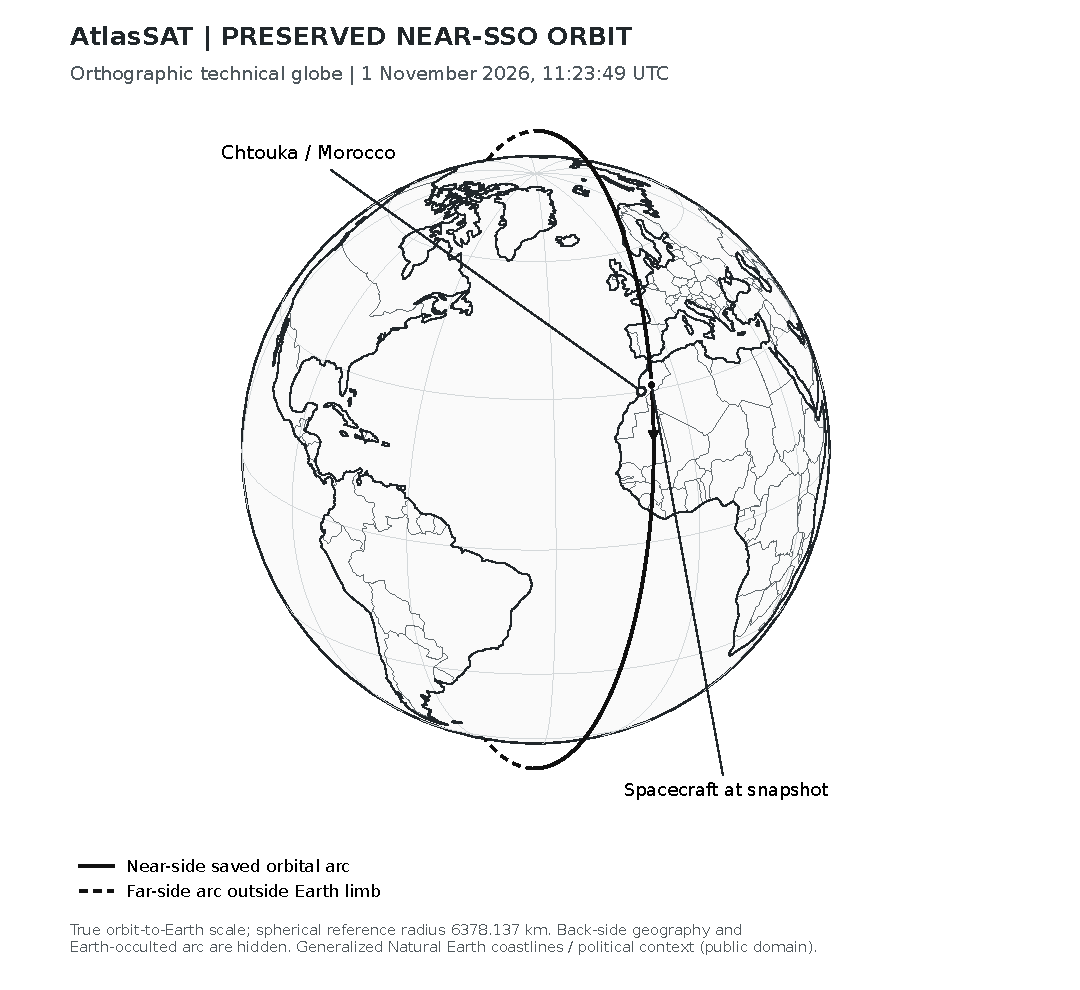
\includegraphics[width=.94\linewidth,height=.73\textheight,keepaspectratio]{08_Technical_Orbital_Globe.pdf}
\caption{Approved monochrome orthographic globe. The preserved near-SSO arc uses a single snapshot orientation at 1 November 2026, 11:23:49 UTC; altitude is not exaggerated. Earth-occulted arc segments and back-side geographic boundaries are hidden; visible far-side segments outside the limb are dashed. The surface marker identifies Chtouka context, separate from the spacecraft marker. Predicted Earth orientation and a spherical display do not establish physical geolocation accuracy. E11/E14; Natural Earth public-domain geographic context.}\label{fig:globe}
\end{figure}
\clearpage
\section{Time, Earth orientation and coordinates}
GMAT input spacecraft elements are expressed in EarthMeanOfDate/MODEq, whereas exported inertial OEM states are Earth-centred EME2000. Orbital-element values in these axes cannot be compared without their epoch-dependent transformations. For terrestrial geometry, the v0.4 post-processor applies a SOFA/ERFA mean-J2000 to GCRS/ICRF frame-bias correction and a SPICE J2000-to-ITRF93 time-dependent six-state transform, including the velocity term associated with rotation. UTC elapsed seconds are accumulated in TT then transformed to TDB/ET as required for SPICE evaluation.

The acquired Earth PCK \texttt{earth\_000101\_270116\_261020.bpc} supplies Earth orientation for 2000--2027; its \emph{last source input} was 20 October 2026 00:00 UTC, before the first simulated epoch. Subsequent dates in the study therefore use \textbf{predicted} orientation, not measured future UT1/EOP. The old and new orientation/frame procedures yield terrestrial position differences up to \textbf{103.00 m} (RMS 67.70 m) for identical inertial states; the frame-bias change by itself was \(\le0.78\) m at tested times. The matched opportunity-boundary shift across 28 targets is \(\le2.872\) ms, and a matched 1 km grid comparison changed mean 72 h area fraction by \(\le0.0152\) percentage point. Differences between model versions are not truth-error bounds.\ev{E06 kernel coverage, \texttt{combined\_full\_orbit\_position}, \texttt{geographic\_event\_comparison} and paired-grid comparison}

\begin{warnbox}
\textbf{Interpretation control.} The approximately microsecond event-root residuals and millimetre/centimetre state comparisons are numerical accuracy diagnostics. They do not establish precision ground geolocation, physical imaging instant, operational UT1, or validated orbit knowledge. Solar elevation is evaluated geometrically without terrain, atmospheric refraction or cloud screening.
\end{warnbox}

\clearpage
\section{Geographic region of interest and evidence quality}
\subsection{Outer boundary, mask and source classes}
The seven selected community/OSM administrative commune polygons cover \textbf{1,173.917 km\textsuperscript{2}}, comprising A\"it Amira, Belfa\^a, Biougra, Inchaden, Massa, Oued Essafa and Sidi Bibi. Names/codes were checked against the 2024 Moroccan HCP commune identities; this verifies identity, not the exact official vertices. Figure~\ref{fig:roi} shows the actual geographic definition. The seven-commune union is an explicit \emph{study boundary}, not an official irrigation-service or aquifer perimeter. No reusable ORMVASM/ABH-SM/CRTS polygon or dated local crop inventory was obtained; the HCP check verifies identities only.

The screened primary agricultural research mask is \textbf{396.472 km\textsuperscript{2}}: temporary-crop source support 261.79 km\textsuperscript{2}, mapped greenhouse support 129.28 km\textsuperscript{2}, and OSM orchard support 5.40 km\textsuperscript{2}. It combines 2021 ESA WorldCover and WorldCereal, a 2020 Global-PCG-10 greenhouse layer, OSM, and a documented October 2026 Sentinel-2 visual screen. The 456.37 km\textsuperscript{2} candidate and 568.05 km\textsuperscript{2} expanded alternatives reflect classification uncertainty rather than certified hectares cultivated in 2026.


\begin{figure}[p]\centering
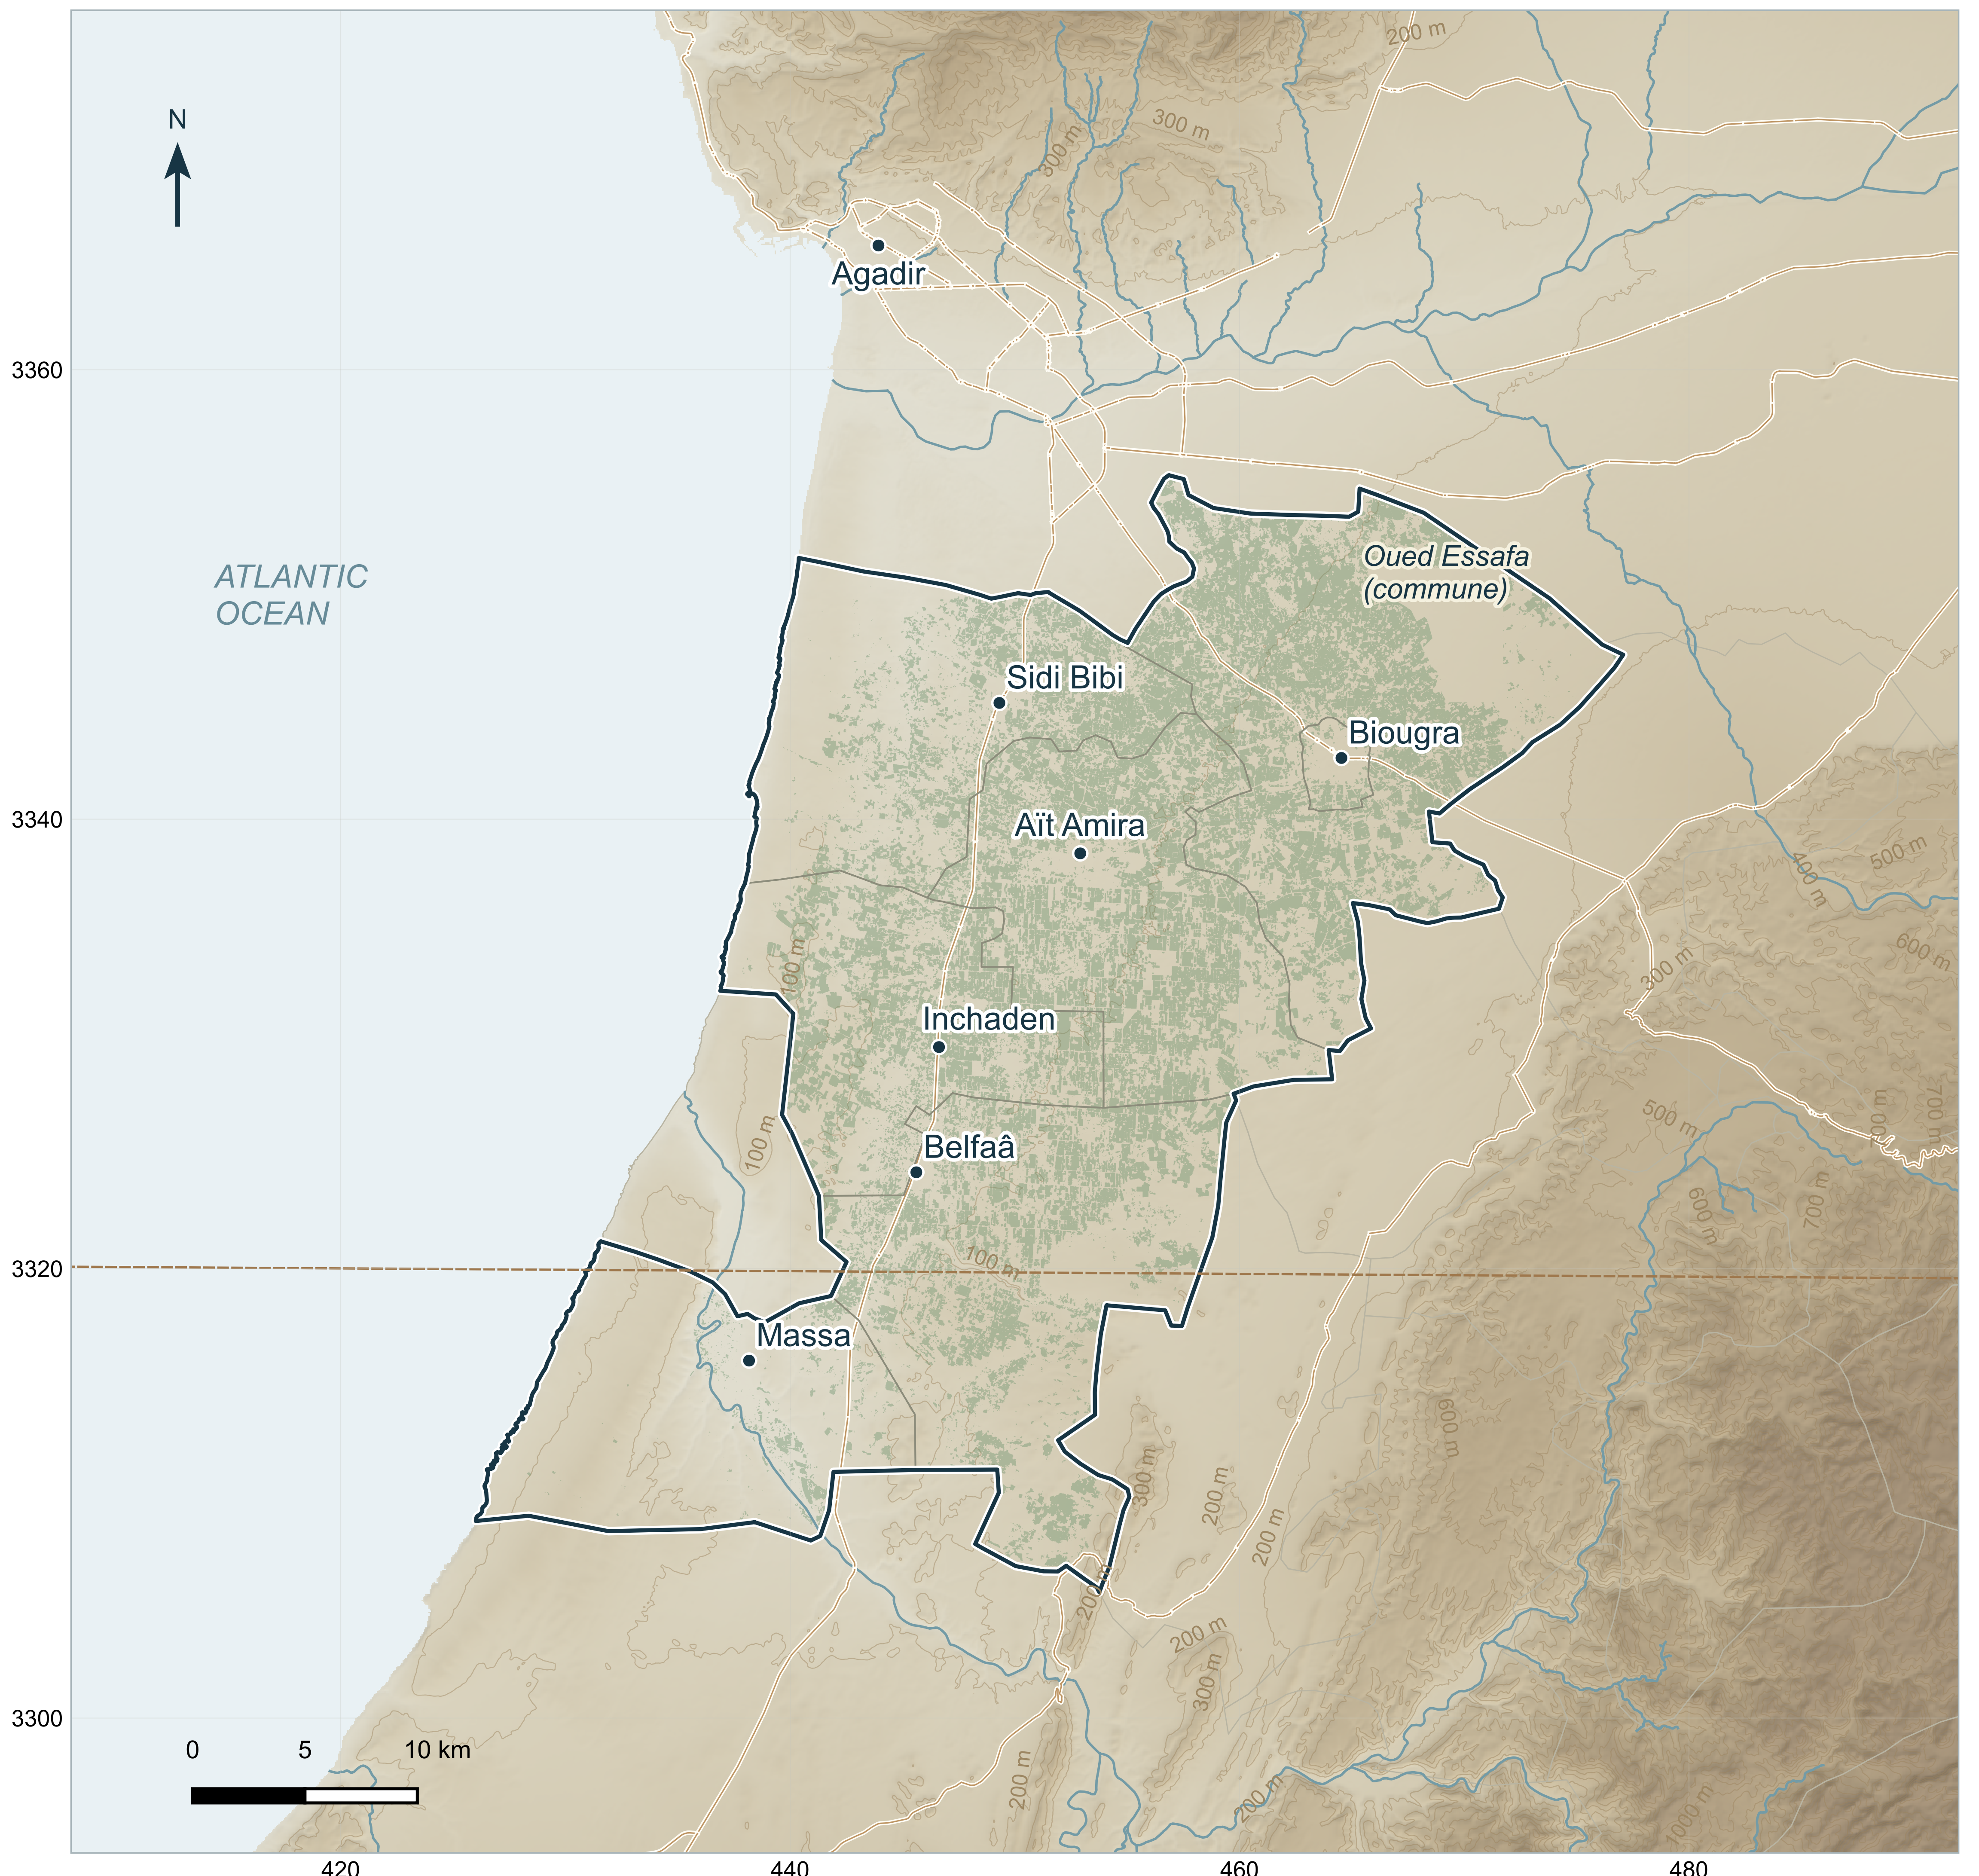
\includegraphics[width=\linewidth]{07_Technical_Atlas_main_600dpi.png}
\par\vspace{2mm}
\begin{minipage}[t]{.66\linewidth}
\vspace{0pt}
\includegraphics[width=99mm]{07_Technical_Atlas_legend_600dpi.png}
\end{minipage}\hfill
\begin{minipage}[t]{48mm}
\vspace{0pt}
{\fontsize{8}{10}\selectfont\bfseries MOROCCO*}\par
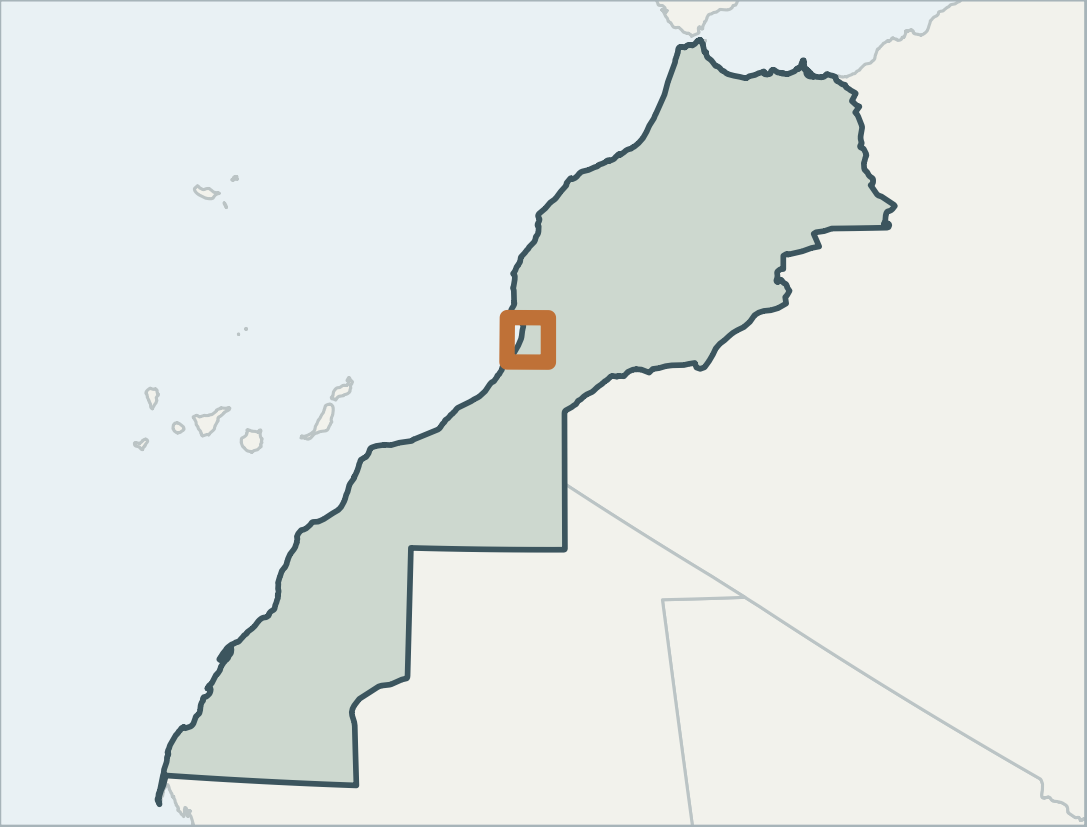
\includegraphics[width=46mm]{07_Technical_Atlas_locator_600dpi.png}
\end{minipage}
\caption{Accepted Technical Atlas, using unchanged crops of its 600 dpi export: detailed OSM land/sea separation, Copernicus DSM relief and the refined Natural Earth locator. The seven-commune boundary and primary mask are unchanged, provisional research geometry. The dashed line marks the southern greenhouse-source limit. *The Morocco locator follows this publication's outline convention; geographic context only. WGS84 / UTM 29N display, original LAEA area measurement. OSM (ODbL); ESA/PCG (CC BY); Copernicus; Natural Earth (public domain). E02/E08/E10/E14.}\label{fig:roi}
\par{\fontsize{6.5}{8}\selectfont\color{atlasgray}Relief produced using Copernicus WorldDEM-30 \copyright\ DLR e.V. 2010--2014 and \copyright\ Airbus Defence and Space GmbH 2014--2018, provided under COPERNICUS by the European Union and ESA; all rights reserved.\par}
\end{figure}
{\fontsize{9}{12}\selectfont\par\Needspace{6\baselineskip}\begin{minipage}{\linewidth}\captionsetup{hypcap=false}\captionof{table}{Study and agricultural areas by commune}\label{tab:areas}\end{minipage}\par\nobreak
\begin{tabularx}{\linewidth}{@{}Xrr@{}}\toprule\rowcolor{headerbg}Commune & Outer area, km$^2$ & Primary mask, km$^2$\\\midrule
A\"it Amira & 176.18 & 90.15\\\rowcolor{rowalt}Belfa\^a & 229.58 & 67.65\\Biougra & 10.63 & 2.56\\\rowcolor{rowalt}Inchaden & 143.04 & 57.63\\Massa & 167.88 & 6.47\\\rowcolor{rowalt}Oued Essafa & 271.28 & 126.39\\Sidi Bibi & 175.33 & 45.64\\\bottomrule\end{tabularx}}
\shortcap{Rounded per-commune values do not necessarily sum to the higher-precision spatial union exactly. E02 gives exact class and subregion areas; E08 confirms administrative identities, not surveyed boundary accuracy.}
\subsection{Regional context and locator convention}
The accepted Technical Atlas remains focused on Chtouka-Massa. Its relief transparency uses full-detail OSM land polygons on the unchanged 60 m grid; the terrain colours, multidirectional hillshade and 100 m contours derive from Copernicus DEM. Roads, rivers and verified locality nodes are OSM context; Oued Essafa is an italic commune-area label rather than an asserted settlement point. The small locator uses Natural Earth 1:10 million country geometry, following this publication's Morocco outline, with matching faint country context. These are traceable cartographic sources, not authoritative boundary or shoreline surveys. Coastline/generalization differences are not used to clip or relabel the mission mask. The national locator retains the regional study marker and the established publication outline; it does not set the mission-area denominator. No official provincial survey or agricultural perimeter is implied.\ev{E14 accepted-asset manifest and source notes; OSM contributors, ODbL 1.0; Natural Earth public domain; Copernicus DEM licence. E12 is retained as historical RevD2 context, not the active map source}





\subsection{Missing southern greenhouse coverage}
The acquired Global-PCG-10 archive provides no corresponding source tile for the relevant study land south of approximately \(30^\circ\)N. Source-absent portions amount to \textbf{258.695 km\textsuperscript{2}} (\textbf{22.04\%}, rounded from 22.037\%) of the outer study boundary and \textbf{27.201 km\textsuperscript{2}} (6.861\%) of the existing primary mask, affecting Belfa\^a and Massa. The candidate and expanded masks have 38.203 and 56.974 km\textsuperscript{2} respectively outside the source footprint. Those areas are \emph{not} estimates of missing greenhouse acreage: unrepresented greenhouses could exist inside or outside the identified agricultural masks. The 2020 greenhouse raster and 2021 crop maps are not a validated 2026 crop census.\ev{E08 native source footprint and equal-area intersections; E02 source vintages and mask totals}



\clearpage
\begin{landscape}
\begin{figure}[p]\centering
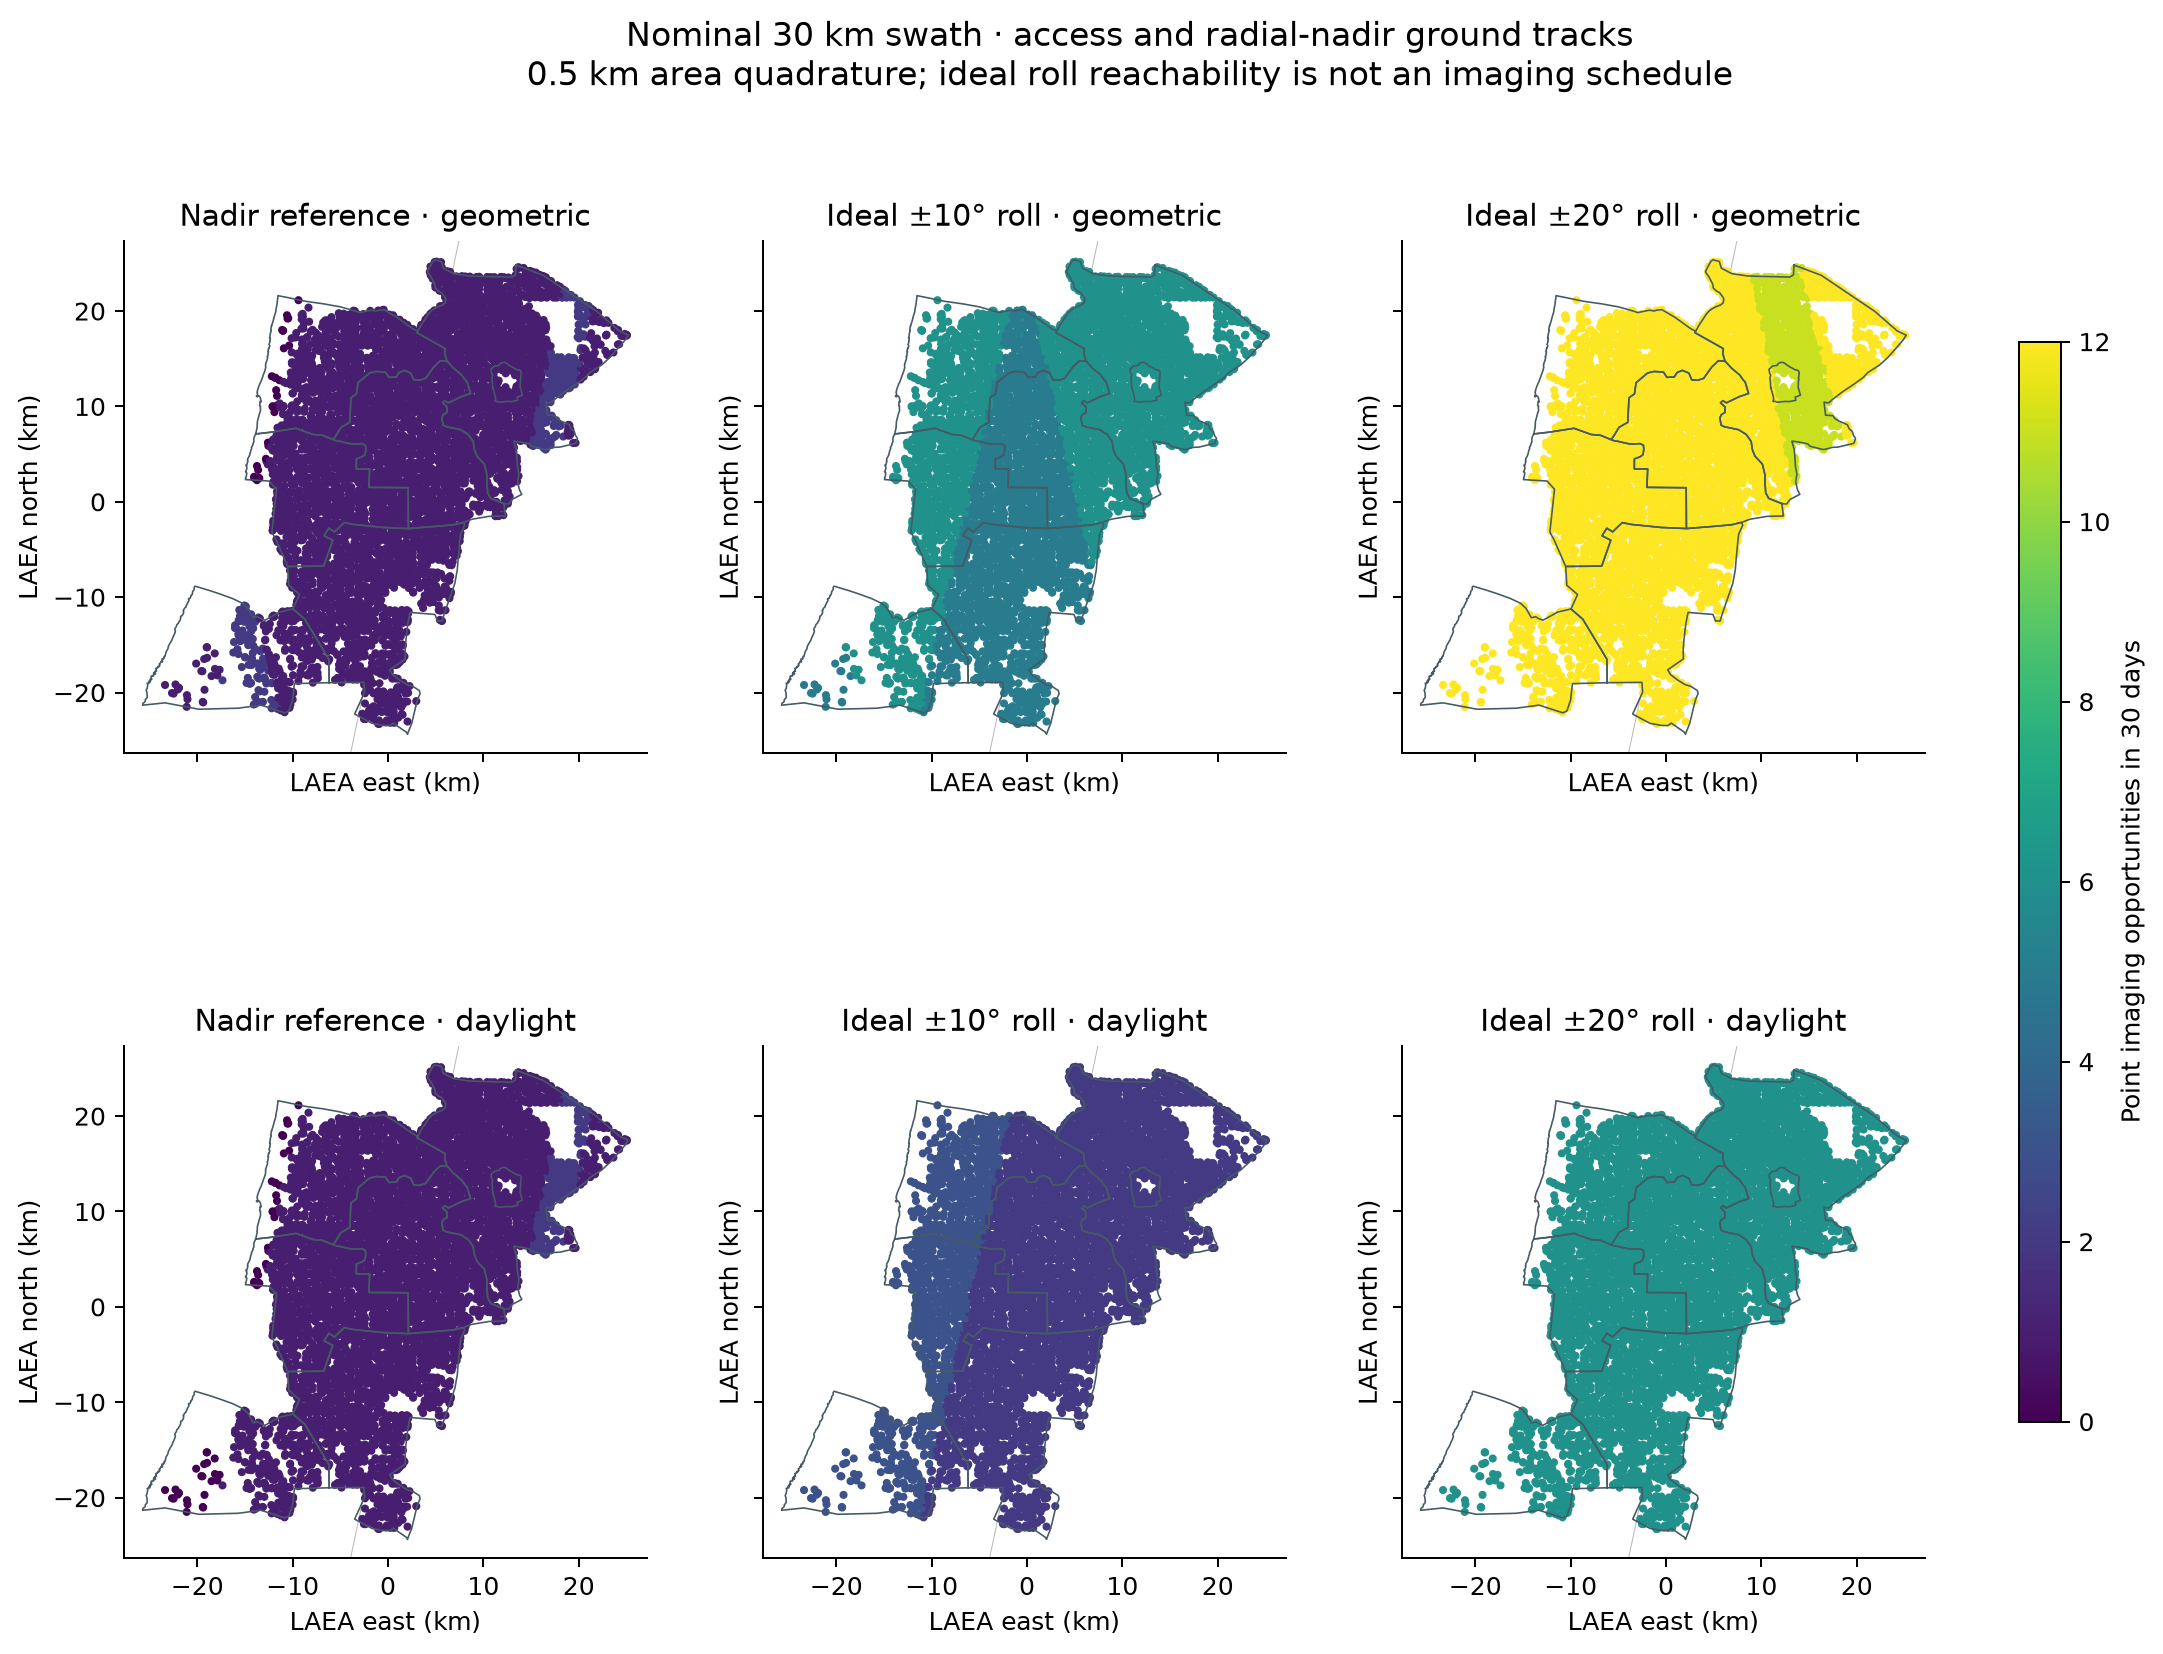
\includegraphics[width=.98\linewidth,height=.79\textheight,keepaspectratio]{02_access_and_tracks.png}
\caption{Original v0.4 access and ground-track figure, reproduced without data changes. Rows separate geometric reachability from daylight opportunities; columns separate nadir and ideal roll envelopes. The underlying map uses 500 m area quadrature, whereas principal coverage tables use 250 m. The radial-nadir track overlays are illustrative 30 s polylines; access events use continuous root refinement, not those plotted samples. Colour gives per-target opportunity count over the saved month, not acquired images. E03/E10; frozen \texttt{revisit\_primary\_500m.csv} and \texttt{groundtrack\_30s.csv}.}\label{fig:tracks}
\end{figure}
\end{landscape}
\clearpage
\section{Imager footprint and event modelling}
\subsection{Pushbroom geometry}
With nominal altitude \(h=550\) km and nadir swath \(W=30\) km, a planar estimate for the full cross-track angular field of view is
\begin{equation}
\theta_{\rm cross}=2\tan^{-1}\left(\frac{W/2}{h}\right)=3.124449834^\circ.
\end{equation}
The provisional 10 m along-track surface sample yields a full along-track angular slit of \(2\tan^{-1}[(0.010/2)/550]=0.001041741^\circ\). Figure~\ref{fig:tracks} illustrates the resulting observation corridors. The model treats the target and spacecraft as continuous geometric points; at the reported ground-relative speed the corresponding point residence windows are approximately \(1.412\)--\(1.559\) ms. This does \emph{not} establish detector IFOV, commanded line rate, charge integration time, achieved GSD, multispectral alignment, modulation-transfer function or signal-to-noise performance.

\begin{figure}[H]\centering
\begin{tikzpicture}[>=Latex,scale=0.9]
\fill[atlasblue!8] (-5,-0.2) rectangle (5,0.15);
\draw[atlasgray,thick] (-5,0.15)--(5,0.15);
\node[below,font=\footnotesize] at (3.3,0.05) {Local ground plane (schematic)};
\node[draw,rounded corners,fill=atlasblue!15,minimum width=1.05cm,minimum height=0.36cm,font=\footnotesize] (sat) at (0,3.45) {AtlasSAT};
\draw[atlasblue,thick,->] (sat.south)--(0,0.26);
\draw[atlasbluelight,dashed] (sat.south)--(-1.75,0.23);
\draw[atlasbluelight,dashed] (sat.south)--(1.75,0.23);
\draw[atlasbluelight,thick,decorate,decoration={brace,amplitude=4pt}] (-1.75,0.34)--(1.75,0.34);
\node[font=\footnotesize,fill=white] at (0,0.6) {30 km nominal cross-track};
\draw[->,very thick,atlasgreen!60!black] (0.25,2.7)--(1.55,2.7);
\node[font=\footnotesize,above] at (2.05,2.72) {Along-track motion};
\node[font=\footnotesize,fill=white] at (-1.0,2.0) {$\theta_{\rm cross}$};
\node[font=\footnotesize,align=center] at (3.5,2.2) {Ideal roll extends\\single-target reach};
\end{tikzpicture}

\caption{Conceptual viewing geometry, not to scale. The pushbroom's 10 m along-track slit is not resolvable in this drawing. A roll envelope describes independently reachable points, not executable slews or simultaneous coverage.}
\end{figure}

\subsection{Coordinate basis and access predicate}
In ITRF93, let target position be $\boldsymbol q$, spacecraft state $(\boldsymbol r,\boldsymbol v)$ and line of sight $\boldsymbol\ell=\boldsymbol q-\boldsymbol r$. Radial nadir and ground-relative horizontal axes are
\begin{equation}
\boldsymbol n=-\frac{\boldsymbol r}{\|\boldsymbol r\|},\quad
\boldsymbol u=\frac{\boldsymbol v-(\boldsymbol v\cdot\boldsymbol n)\boldsymbol n}{\|\boldsymbol v-(\boldsymbol v\cdot\boldsymbol n)\boldsymbol n\|},\quad
\boldsymbol c=\boldsymbol u\times\boldsymbol n.
\end{equation}
With $d=\boldsymbol\ell\cdot\boldsymbol n$, $x=\boldsymbol\ell\cdot\boldsymbol c$, $y=\boldsymbol\ell\cdot\boldsymbol u$, and full FOV half-angles $\theta_c=\theta_{\rm cross}/2$, $\theta_a=\theta_{\rm along}/2$, the implementation uses
\begin{equation}
\alpha=\operatorname{atan2}(x,d),\quad
\rho=\operatorname{clip}(\alpha,-\rho_{\max},+\rho_{\max}),\quad
\beta=\operatorname{atan2}(y,d\cos\rho+x\sin\rho).
\end{equation}
Access requires surface visibility $\boldsymbol n_g\cdot(\boldsymbol r-\boldsymbol q)>0$, $|\alpha|\le\rho_{\max}+\theta_c$, and $|\beta|\le\theta_a$. Setting $\rho_{\max}=0$ gives the nadir reference. The roll-dependent denominator is retained; this is not a sample-only or circular-footprint test. Each point's ideal roll is selected separately, so these predicates do not constitute an executable common pointing schedule.\ev{E10 METHOD/config; frozen v0.4 \texttt{src/coverage.py}}

\subsection{Continuous event detection}
For irregular or widely spaced Cartesian ephemeris samples, the saved v0.4 pipeline uses position--velocity cubic Hermite interpolation and signed along-track fan-plane roots to find short target crossings between 30 s OEM records. Given endpoints \((\boldsymbol r_0,\boldsymbol v_0)\), \((\boldsymbol r_1,\boldsymbol v_1)\), \(u=(t-t_0)/\Delta t\), the standard interpolant is
\begin{multline}
\boldsymbol r(u)=(2u^3-3u^2+1)\boldsymbol r_0+(u^3-2u^2+u)\Delta t\,\boldsymbol v_0\\
+(-2u^3+3u^2)\boldsymbol r_1+(u^3-u^2)\Delta t\,\boldsymbol v_1.
\end{multline}
\ev{E10 METHOD; angular FOV is a derived geometric estimate, not a verified instrument specification}
The pipeline brackets fan-plane crossings, refines angular entry/exit roots and clips visibility/cross-track boundaries. A 30 s \emph{sample-in-footprint} check cannot reliably discover millisecond point windows; discovery and refinement are verified separately against the saved independent checks (E05).

\subsection{Daylight interpretation}
If \(\boldsymbol s\) is the unit target-to-Sun direction and \(\boldsymbol n_g\) the outward ellipsoid normal at the target, geometric solar elevation is \(E_\odot=\arcsin(\boldsymbol n_g\cdot\boldsymbol s)\). Optical daylight opportunities require \(E_\odot\ge0^\circ\), with a separate \(10^\circ\) sensitivity gate. Terrain shadow, cloud cover, seasonal crops and illumination-dependent image quality were not evaluated. Individual point windows do not represent the time necessary for full image-strip acquisition and spacecraft slew/settle.

The methodological companion is \href{AtlasSAT_2A-2_Analytical_Derivations_v0.2.1_Public_RC_v0_2.pdf}{\emph{Document 2A-2 --- Analytical Derivations \& Independent Verification}}, v0.2.1 (49 pages, 27 October 2026; E18). It supplies step-by-step derivations, analytical predictions/approximations and independent consistency comparisons with archived GMAT/Python outputs, including assumptions, residuals and verification limits. It does not establish flight qualification or physical/operational mission validation.

\analref{Chs.~6--8, Eqs.~(6.1)--(6.3), (7.3)--(7.10), (8.1)--(8.5), Tables~26--28} derives pushbroom footprint, LOS/roll, illumination and event-boundary geometry, with worked local checks of millisecond point windows rather than an exhaustive ROI search. GMAT supplies native propagation and ephemeris export; Python performs agricultural optical-access, illumination and revisit analysis.

\subsection{Illustrative passages from the preserved trajectory}
Figures~\ref{fig:globe} and~\ref{fig:passages} connect the preserved near-SSO orbit to the agricultural study. Event 1 is a saved nominal-swath nadir access to \emph{Massa} on 24 October at approximately 22:51:42 UTC, with target Sun elevation $-62.32^\circ$: geometric access at night. Event 2 is a corresponding \emph{Oued Essafa} sample on 1 November at approximately 11:23:49 UTC, with Sun elevation $+43.13^\circ$: a daylight opportunity, without a claim of usable acquired imagery. Event 3 is the radial central ground track inside the outer study boundary in two intervals within 16 November 11:24:31--38 UTC. It is a boundary-crossing diagnostic, not a full-ROI acquisition.

Exact selected point IDs, entry/exit times, source CSV lines and raw-file hashes are in E11. These are examples selected from existing results, not a new access or revisit calculation. The monochrome globe uses a single snapshot orientation at event 2; the regional panels use each date's terrestrial trajectory and separate illumination classification. Dates are not simultaneous states.\ev{E11 raw event selection and direct SPICE solar-sign checks; E10 radial-nadir convention. Numerical UTC precision is not physical event-time accuracy}
\clearpage
\newgeometry{top=12mm,bottom=12mm,left=12mm,right=12mm}
\begin{landscape}
\thispagestyle{empty}
\begin{figure}[p]\centering
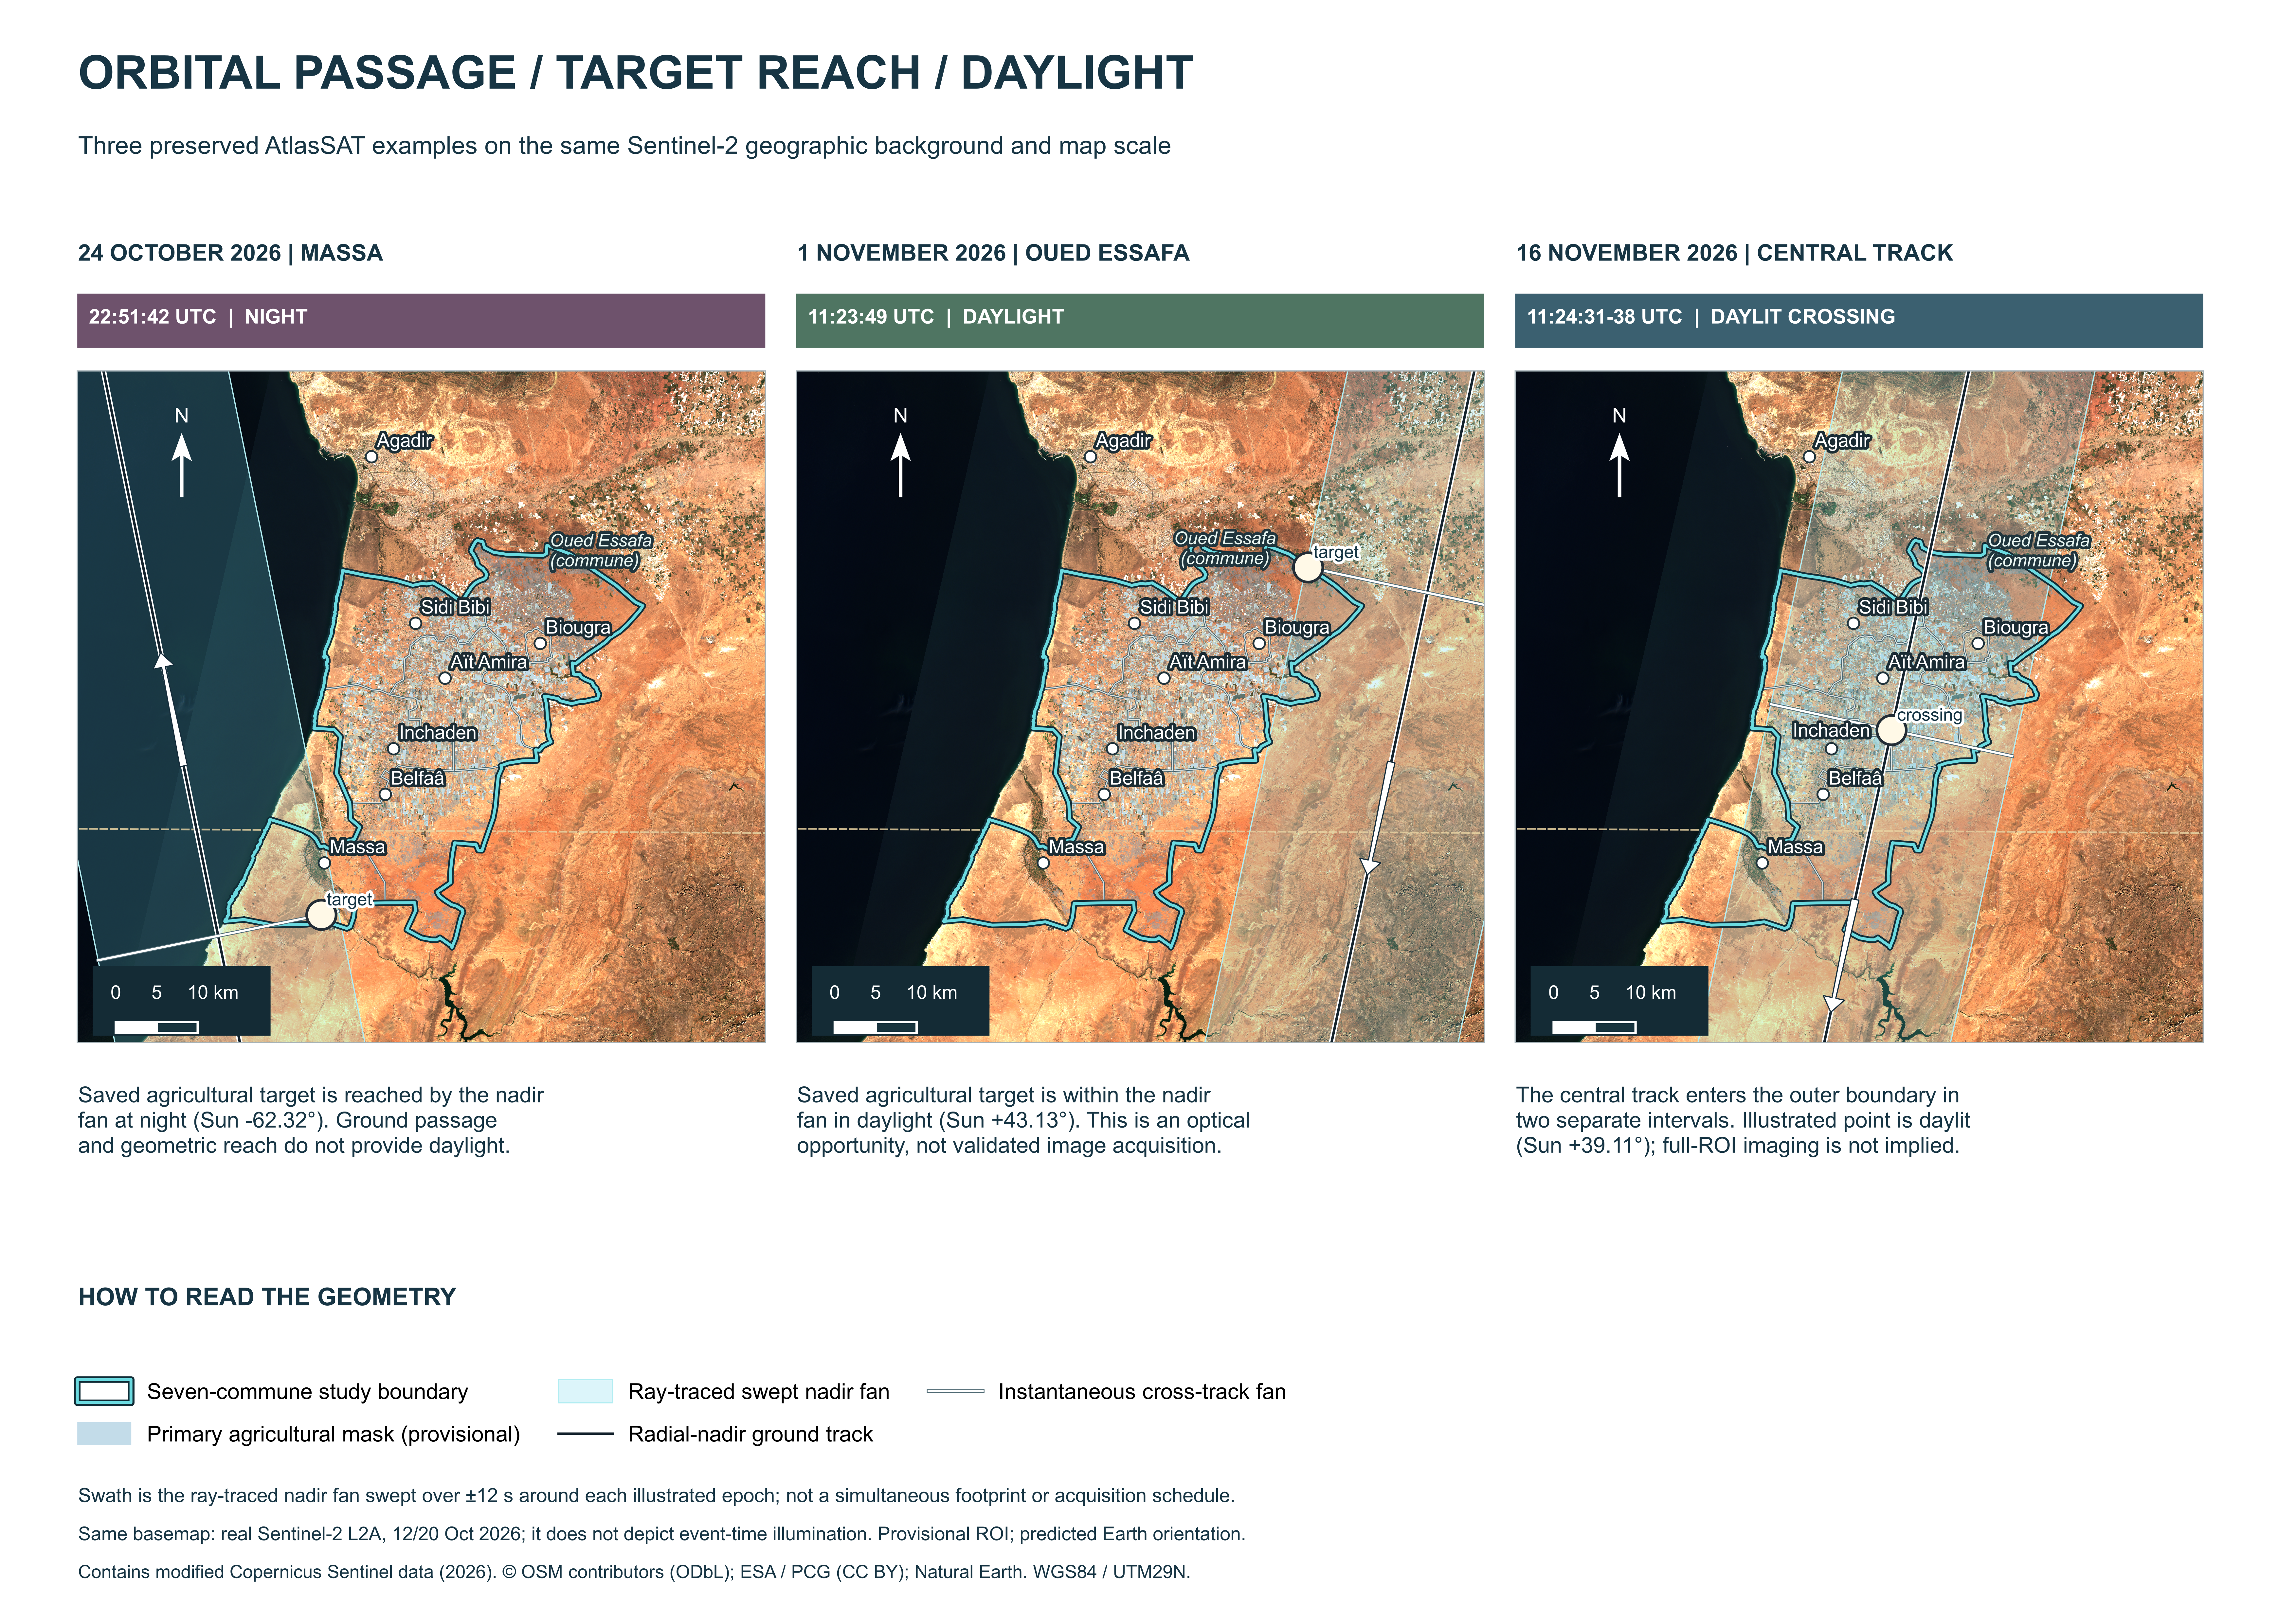
\includegraphics[width=.96\linewidth,height=.90\textheight,trim=8mm 3mm 8mm 27mm,clip,keepaspectratio]{09_Three_Orbital_Passages.png}
\caption{Three separate epochs on the same Sentinel-2 background and map scale: Massa night access, Oued Essafa daylight opportunity, and a central-track boundary crossing. The shaded corridor is a ray-traced nadir fan swept around each event, not a simultaneous footprint or executable image strip. The imagery does not depict event-time illumination. Provisional ROI; predicted orientation; OSM (ODbL), ESA/PCG (CC BY), modified Copernicus Sentinel data and Natural Earth. E11/E14.}\label{fig:passages}
\end{figure}
\end{landscape}
\restoregeometry
\clearpage
\section{Coverage, revisit and requirement decision}
\subsection{Metrics and censoring}
For target \(j\) with qualifying access intervals \([s_{j,k},e_{j,k}]\), complete optical no-access gaps are \(G_{j,k}=s_{j,k+1}-e_{j,k}\). Revisit midpoint differences can also be tabulated but should not be silently substituted for \(G_{j,k}\). Left/right censored spans run from simulation start to first entry and last exit to simulation end; when no access exists the entire 720 h interval is an observed no-access span. These spans are lower bounds on unknown adjacent full intervals. A target with zero access has \emph{undefined}, not zero, complete revisit statistics.

For a time window \([t,t+H]\), the area-weighted sampled coverage fraction is
\begin{equation}
C_H(t)=\frac{\sum_j A_j\,\mathbf1\bigl\{\exists k:\ m_{j,k}\in[t,t+H]\bigr\}}{\sum_j A_j},\qquad m_{j,k}=\tfrac12(s_{j,k}+e_{j,k}),
\end{equation}
where \(A_j\) is each representative cell's \emph{actual agricultural intersection area}. The reported rolling averages use starts every hour over fully contained 24/48/72 h windows, and measure at least one geometric opportunity per sampled agricultural area cell, not an acquired or delivered image.

\subsection{Principal thirty-day result}
{\fontsize{9}{12}\selectfont\par\Needspace{6\baselineskip}\begin{minipage}{\linewidth}\captionsetup{hypcap=false}\captionof{table}{Principal daylight opportunity results}\label{tab:results}\end{minipage}\par\nobreak
\begin{tabularx}{\linewidth}{@{}Xrrr@{}}\toprule\rowcolor{headerbg}30 km / daylight & Nadir & Ideal $\pm10^\circ$ & Ideal $\pm20^\circ$\\\midrule
Mean rolling 24 h agricultural coverage & 3.56\% & 7.42\% & 20.66\%\\\rowcolor{rowalt}
Mean rolling 48 h coverage & 7.38\% & 14.82\% & 28.53\%\\
Mean rolling 72 h coverage & \textbf{11.48\%} & \textbf{22.76\%} & \textbf{33.44\%}\\\rowcolor{rowalt}
Maximum complete daylight gap & 360.01 h & 360.01 h & \textbf{312.22 h}\\
Maximum observed span, incl. censoring & 720.00 h & 360.01 h & 312.22 h\\\bottomrule\end{tabularx}}

\begin{figure}[htbp]\centering
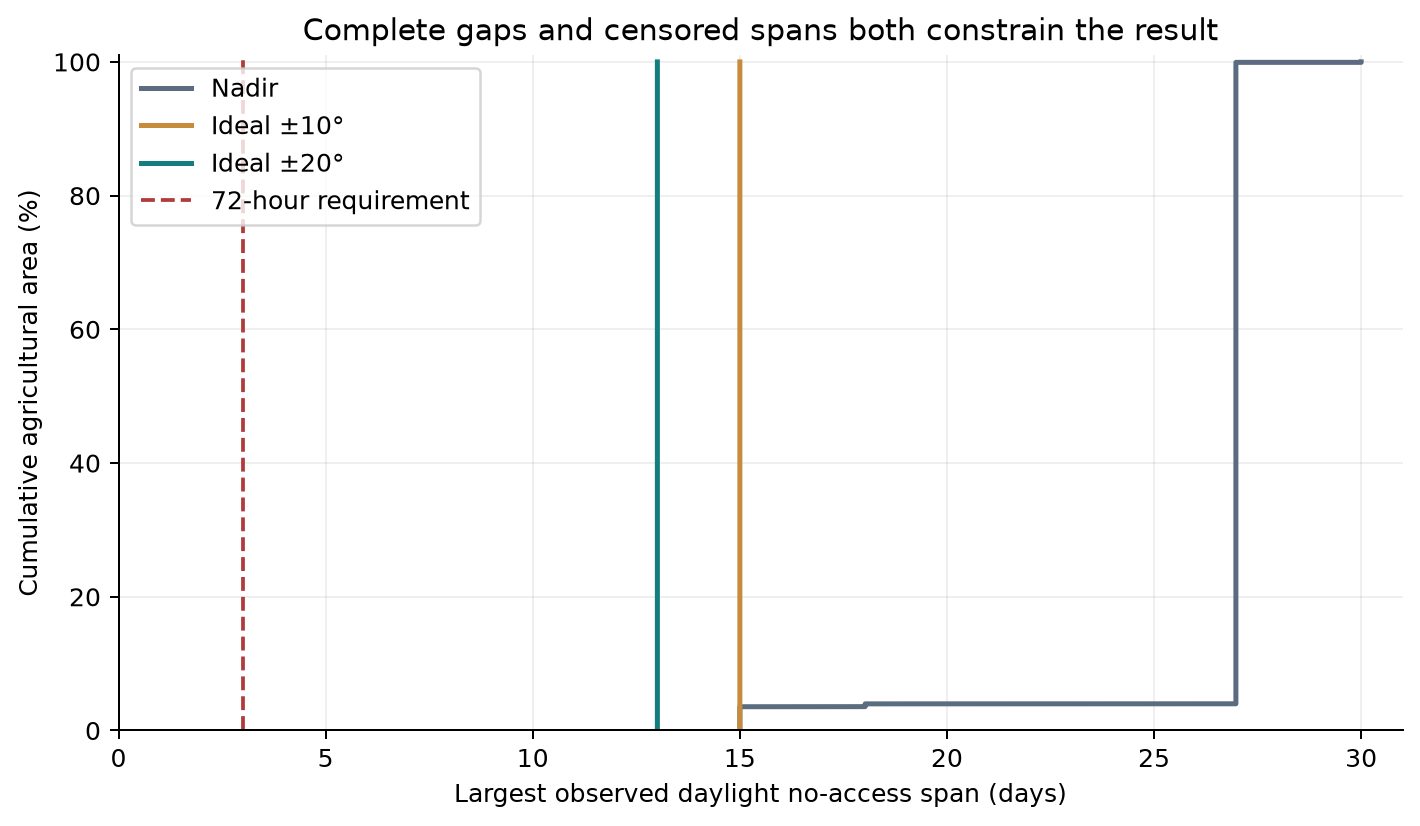
\includegraphics[width=\linewidth]{04_gap_evidence.png}
\caption{Original v0.4 gap-tail evidence, including censored spans. Horizontal position is each target\textquotesingle s largest observed daylight no-access span; the cumulative agricultural area uses its GIS weight. The requirement is 3 days. Nadir includes targets unaccessed throughout the 30-day run, while even ideal $\pm20^\circ$ has gaps near 13 days. This is an opportunity test, not a schedule or image-quality result. E04: \texttt{exact\_window\_summary}; frozen \texttt{exact\_window\_gaps\_primary\_250m.csv}.}\label{fig:gaps}
\end{figure}


Figures~\ref{fig:gaps} and~\ref{fig:rolling} show complementary gap-tail and rolling-coverage evidence. As Figure~\ref{fig:gaps} shows, the long tail remains decisive. The nominal sample contains \textbf{14,494} agricultural quadrature targets at a 250 m spatial resolution. The release reports \textbf{14,494/14,494} with an observed gap above 72 h, including the idealised roll cases. The minimum rolling 72 h coverage is zero in all nominal-swath scenarios. A pooled \(\pm20^\circ\) complete-gap median near 23.90 h cannot establish a \emph{maximum} three-day service: accesses cluster between longer outage intervals.

\ev{E03 rolling-hourly means, failed-target counts and pooled complete revisits; E04 exact exit-to-entry gaps}

\begin{figure}[p]\centering
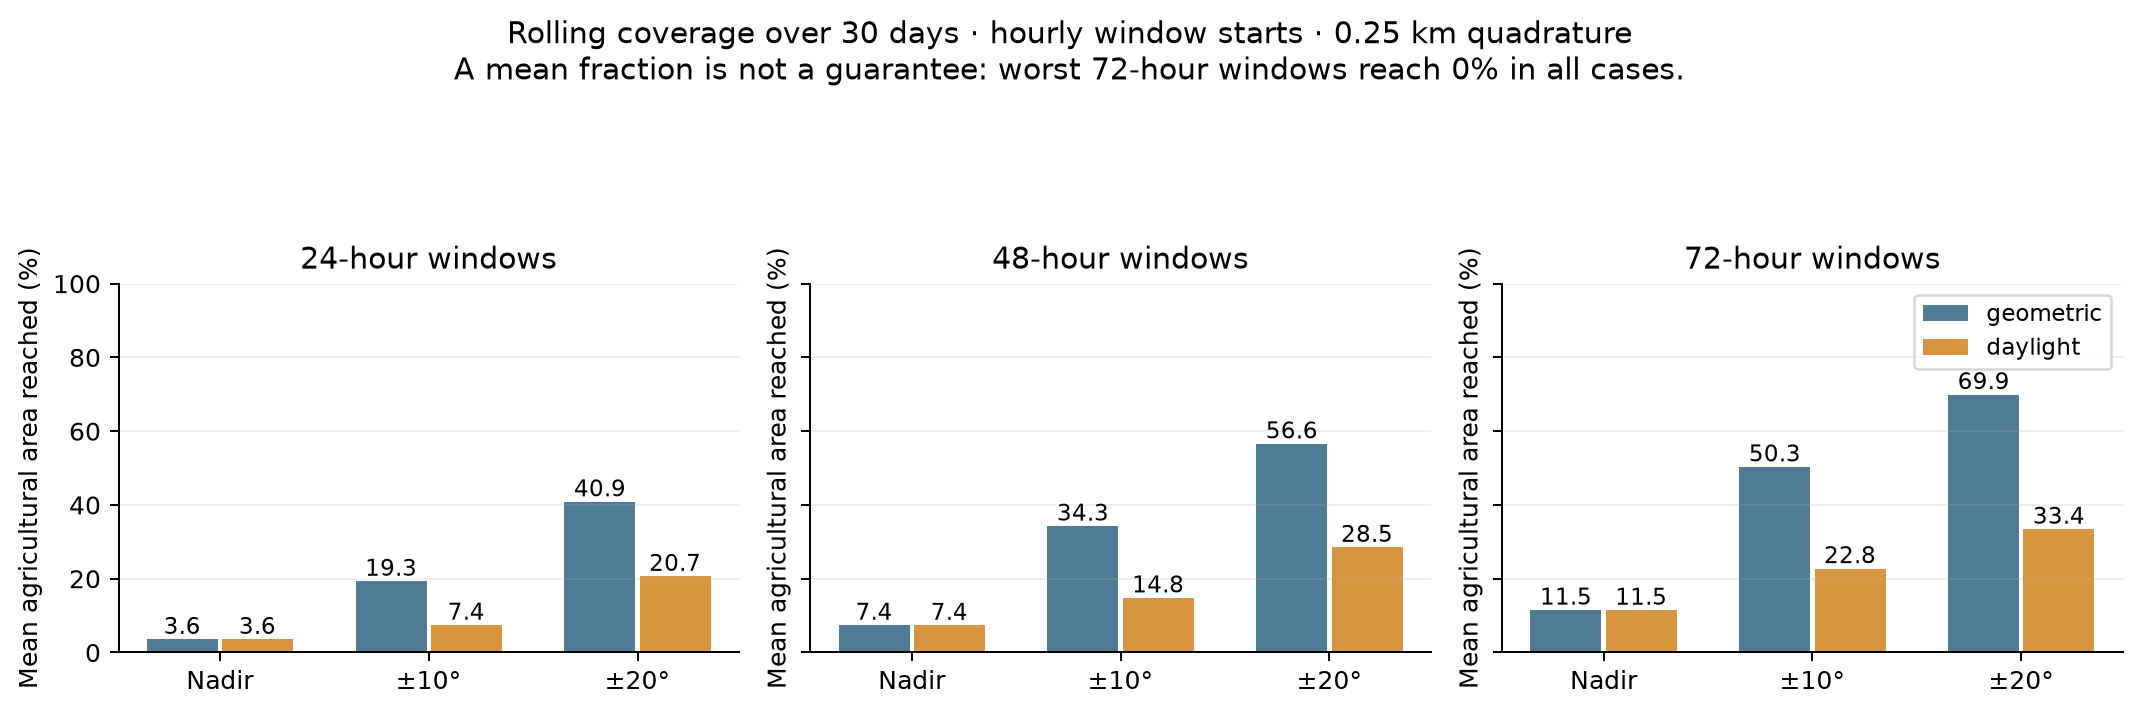
\includegraphics[width=\linewidth]{03_rolling_coverage.png}
\caption{Original v0.4 rolling-coverage summary. The bars compare mean agricultural fractions across rolling 24/48/72 h window lengths and illumination classes; this is not an acquired-imagery timeline. Source values, scenario labels and the 250 m quadrature are unchanged. E03/E10; original figure and source sidecar retained.}\label{fig:rolling}
\end{figure}
\subsection{Worst-case agricultural target --- resolved provenance}
{\fontsize{9}{12}\selectfont\par\Needspace{6\baselineskip}\begin{minipage}{\linewidth}\captionsetup{hypcap=false}\captionof{table}{Worst complete daylight gap: agricultural provenance}\label{tab:worstgap}\end{minipage}\par\nobreak
\begin{tabularx}{\linewidth}{@{}lX@{}}\toprule\rowcolor{headerbg}Evidence field & Confirmed value\\\midrule
Agricultural target ID & \texttt{sidi-bibi\_-10750\_19500} (Sidi Bibi)\\\rowcolor{rowalt}
WGS84 target location & 30.276400208635273$^\circ$N, 9.61006239223738$^\circ$W\\
Previous daylight window exit & 2026-11-02 11:17:35.047317 UTC\\\rowcolor{rowalt}
Next daylight window entry & 2026-11-15 11:30:46.896619 UTC\\
Exact complete no-access gap & \textbf{312.219958139439 h} (13.01 days)\\\rowcolor{rowalt}
Raw evidence & \texttt{results/access\_primary\_250m.csv}, lines 232405/232411\\\bottomrule\end{tabularx}}
The supplementary audit reports that all 14,494 agricultural samples have a gap that rounds to 312.22 h (spread only 0.144 s), associated with the same 2--15 November access-pass pair. Figure~\ref{fig:timeline} shows this pattern; it is \emph{not} proof of an exactly repeating orbit or all-season recurrence. The historical 30.4$^\circ$N / 9.6$^\circ$W reference was explicitly \emph{excluded} from the agricultural aggregate. Its previously similar 312.22 h value differs by about 0.015 s in the exact gap and agrees after rounding.\ev{E07: \texttt{primary\_250m.exact\_maximizers}, raw lines include the header; E08 verifies REF outside the study area}

\begin{warnbox}
\textbf{Optical revisit verdict: NOT MET for the sampled, provisional primary ROI at the inherited initial phase.} Even ideal \(\pm20^\circ\) roll yields a complete no-access interval of 312.22 h, exceeding the 72 h design target by more than a factor of four. No inference that a different orbit, new payload, or scheduled ADCS would meet this requirement has been demonstrated.
\end{warnbox}

\subsection{Agricultural subregion comparison}
{\fontsize{9}{12}\selectfont\par\Needspace{6\baselineskip}\begin{minipage}{\linewidth}\captionsetup{hypcap=false}\captionof{table}{Subregion daylight coverage comparison}\label{tab:subregions}\end{minipage}\par\nobreak
\begin{tabularx}{\linewidth}{@{}Xrrr@{}}\toprule\rowcolor{headerbg}Mean rolling 72 h daylight coverage & Nadir & Ideal $\pm10^\circ$ & Ideal $\pm20^\circ$\\\midrule
A\"it Amira & 11.09\% & 22.22\% & 33.44\%\\\rowcolor{rowalt}
Belfa\^a & 11.09\% & 22.38\% & 33.44\%\\Biougra & 11.09\% & 22.19\% & 33.44\%\\\rowcolor{rowalt}
Inchaden & 11.08\% & 24.22\% & 33.44\%\\Massa & 10.95\% & 24.75\% & 33.44\%\\\rowcolor{rowalt}
Oued Essafa & 12.33\% & 22.19\% & 33.44\%\\Sidi Bibi & 11.06\% & 23.92\% & 33.44\%\\\bottomrule\end{tabularx}}
\shortcap{These ratios apply to each commune's screened agricultural submask; they must not be interpreted as all parcels simultaneously imaged or to imply local greenhouse completeness.}

\ev{E03 subregion coverage; area fractions use each commune\textquotesingle s own screened agricultural submask}

\section{Sensitivity studies and validation}
\subsection{Spatial convergence, classification and swath}
The 250 m primary quadrature has 14,494 on-mask targets; the 500 m and 1,000 m alternatives have 4,254 and 1,262 respectively. For all tested 30 km/roll/illumination combinations, the maximum change in mean 24/48/72 h coverage from 500 to 250 m is reported as \textbf{0.00460 percentage point}. This supports convergence of \emph{area-averaged} opportunity fractions, not proof of every field/edge access. The expanded 568.05 km\textsuperscript{2} research mask shifts mean 72 h coverage by at most 0.1461 percentage point at the matched 1 km grid, without removing sampled revisit failures. The unsimulated 456.37 km\textsuperscript{2} candidate layer has a minor recorded polygon self-intersection; it cannot be presented as an analysis-ready geometry until separately repaired and versioned.

Figure~\ref{fig:swath} retains the saved sensitivity plot. The 20/30/40 km swath sensitivity shows only modest shifts in rolling mean over the same 1 km agricultural grid; the 20 km case is deliberately below the nominal design target. Enlarging angular FOV under fixed orbital conditions does not independently prove acceptable revisit or imager performance.

\ev{E04 spatial convergence and expanded-mask sensitivity; E08 topology diagnostics; E10 findings and saved 1 km summaries}

\begin{figure}[p]\centering
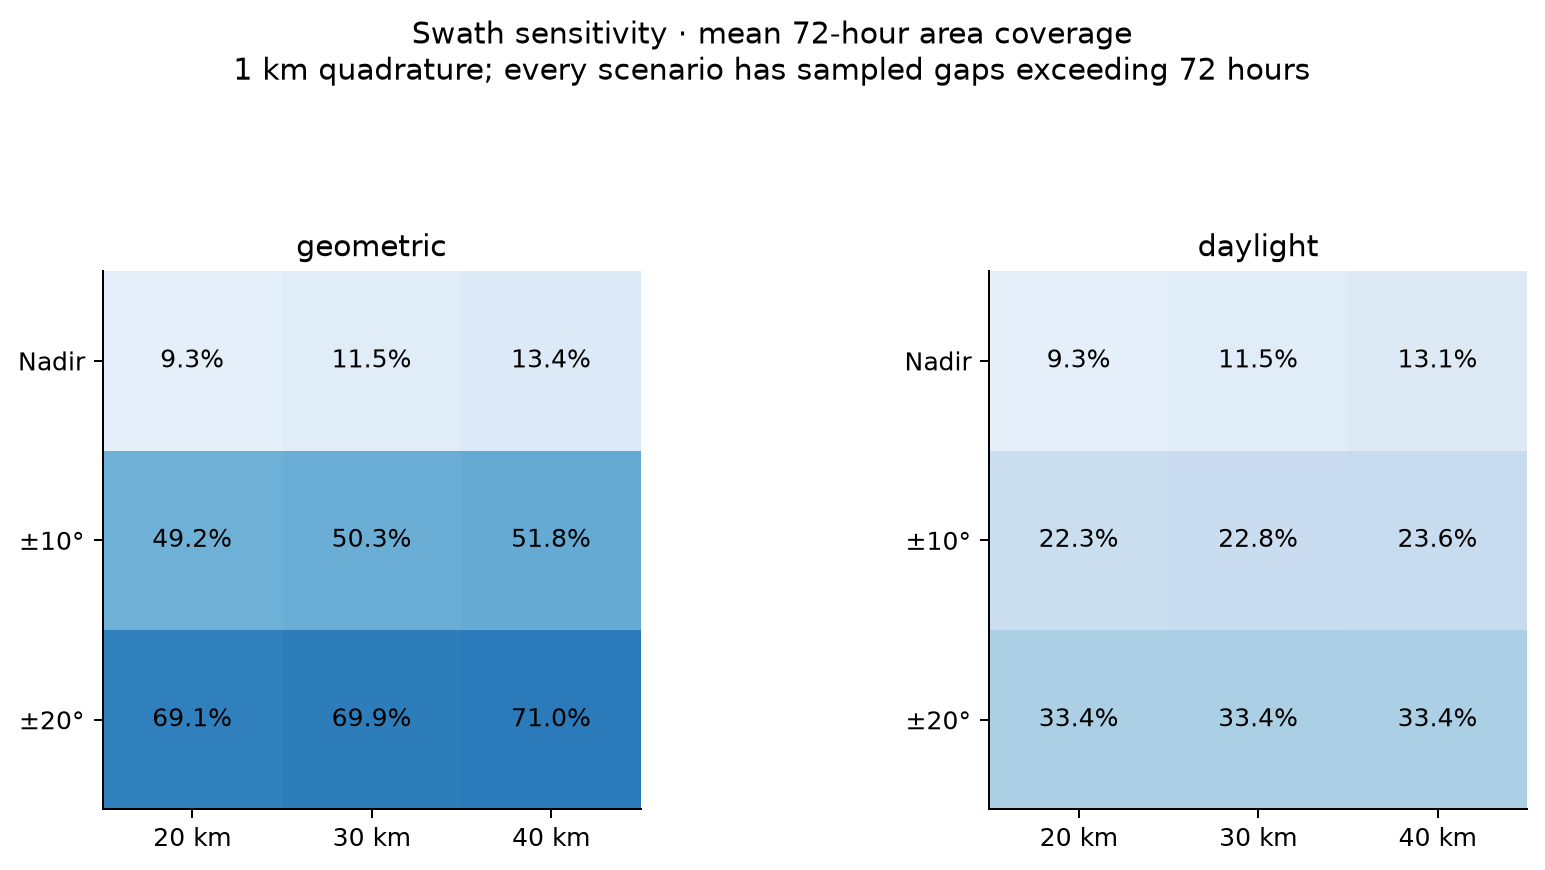
\includegraphics[width=.95\linewidth]{05_swath_sensitivity.png}
\caption{Original v0.4 nominal-swath sensitivity at the matched 1 km grid. The plotted swath and ideal-roll choices are geometric assumptions; none is a demonstrated payload or attitude capability. Changing swath does not by itself establish the maximum daylight-revisit requirement. E04/E10; original figure and source sidecar retained.}\label{fig:swath}
\end{figure}
\subsection{Orbit initial-condition sensitivity --- not a pure phase trade}
Two additional GMAT runs change input true anomaly to 90$^\circ$ and 180$^\circ$ at the same stated osculating semimajor axis, eccentricity and plane. For 30 km and ideal \(\pm20^\circ\) roll, 72 h daylight mean area coverage at 1 km was 33.44\% (0$^\circ$), 0\% (90$^\circ$), and 37.14\% (180$^\circ$). The 90$^\circ$ case yielded geometric opportunities but \emph{only at night}; all 37,860 saved agricultural access instances had target solar elevation from approximately \(-64.85^\circ\) to \(-61.74^\circ\). Independent checks reproduced the Sun elevation signs at tested events.

Figure~\ref{fig:convergence} presents the saved spatial and initial-condition comparison. The final technical review found that \textbf{TA90 also changes subsequent mean orbital period}: mean descending-node period was 95.578336 min at the base phase, 95.967473 min at TA90, and 95.579186 min at TA180. Because J2 makes mean-element correction latitude dependent, holding \emph{osculating} \(a\) fixed does \emph{not} isolate a pure phase change at a common mean orbit. TA90's 15 nodal periods nearly equal 24 h (23.991868 h), helping maintain a repeating night-access corridor. These runs remain useful \emph{initial-condition sensitivities}, not an optimised launch-phase study or a demonstrated route to optical compliance.

\ev{E09 phase periods, direct Sun/frame checks and solar range. TA90\textquotesingle s daytime branch misses the roll envelope; reachable ascending passes occur at night}

\begin{figure}[p]\centering
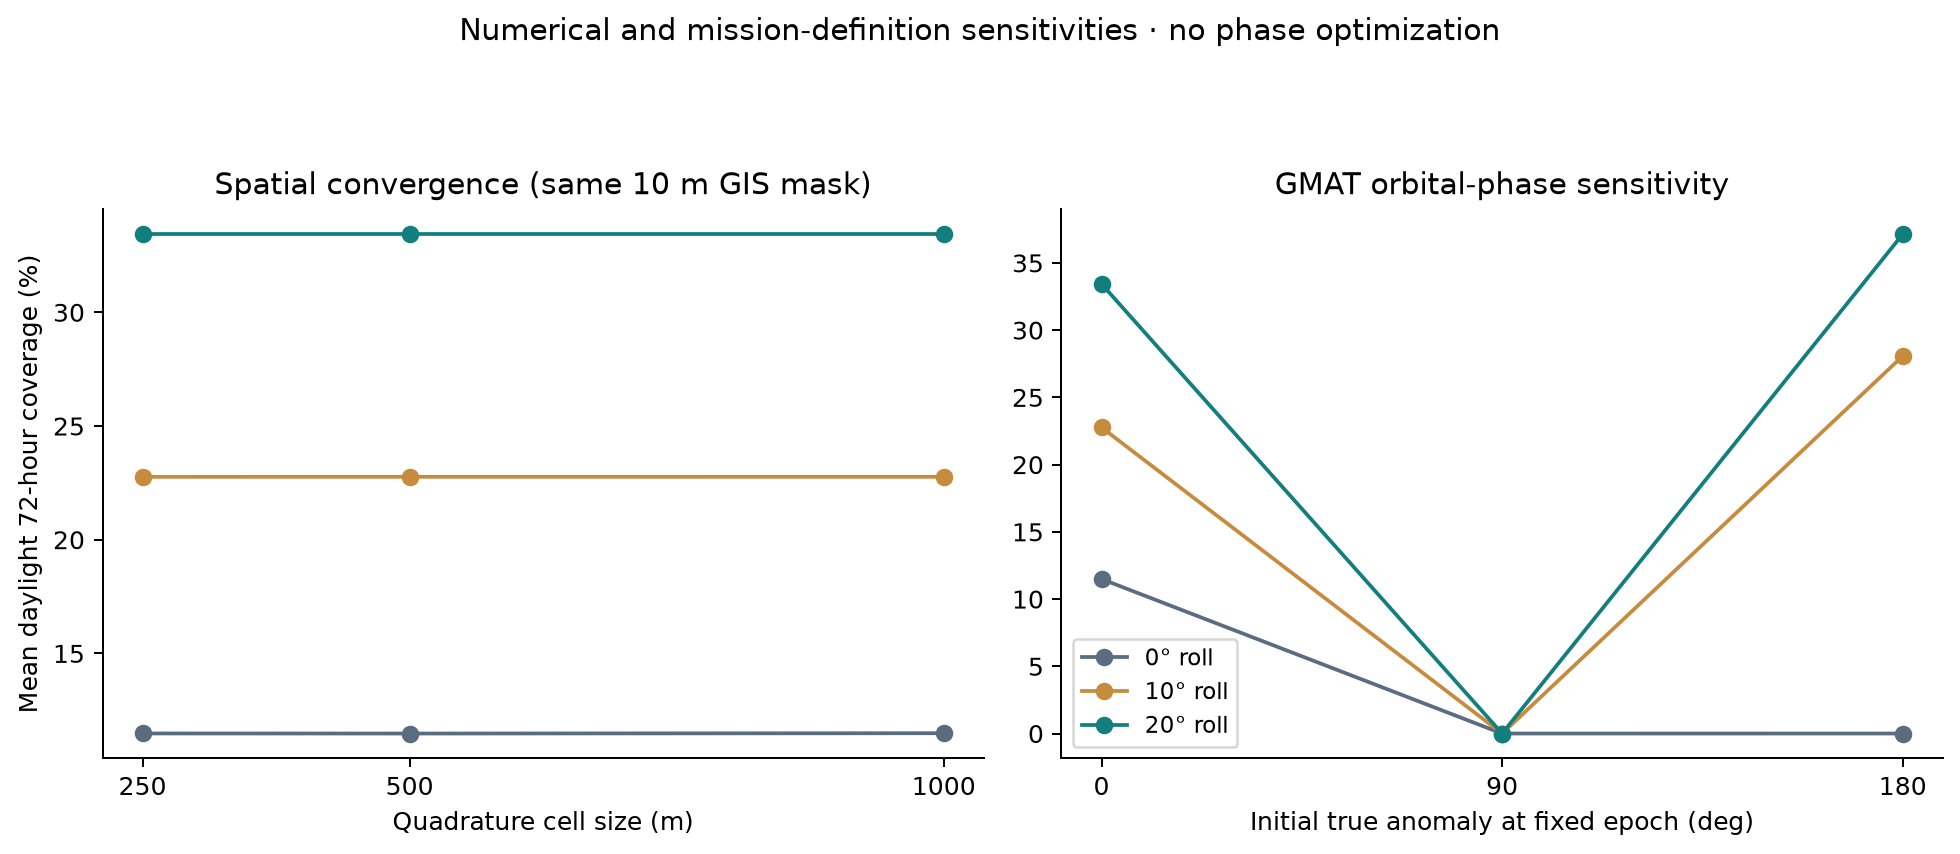
\includegraphics[width=\linewidth]{06_convergence_and_phase.png}
\caption{Original v0.4 spatial-convergence and initial-condition sensitivity figure. Area-mean convergence is numerical evidence, not field-level classification validation. The legacy phase axis denotes changed initial true anomaly at fixed osculating inputs; TA90 also changes the subsequent mean orbit, so it is not a pure phase-only comparison. The night-access explanation and independent solar checks are retained in the text. E04/E09/E10.}\label{fig:convergence}
\end{figure}
\begin{figure}[p]\centering
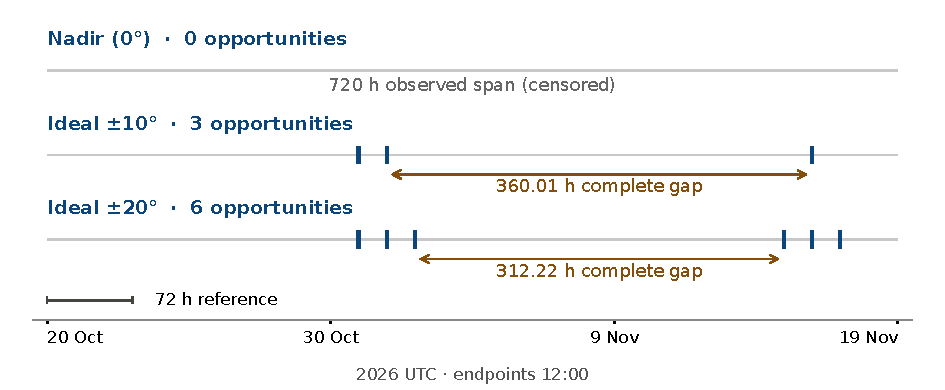
\includegraphics[width=.88\linewidth]{13_Daylight_Timeline.pdf}
\caption{Saved daylight opportunities at \texttt{sidi-bibi\_-10750\_19500}, nominal 30 km swath, 20 October--19 November 2026 (12:00 UTC endpoints). The tracks contain 0, 3 and 6 opportunities. Nadir's 720 h no-access span is censored, not a complete revisit. Arrows mark complete exit-to-next-entry gaps for ideal roll; tick widths do not represent acquisition duration. E16, cross-checked against GUI-first three-target events.}\label{fig:timeline}
\end{figure}
\subsection{Independent geometric checks and preservation}
The v0.4 investigation reports an independent inertial Lagrange/direct-SPICE reference matching \textbf{570} opportunities across 31 geographically distributed targets and three roll scenarios, with maximum entry/exit discrepancy \textbf{1.197 $\boldsymbol\mu$s}. The evidence also includes 468 forward ray/ellipsoid boundary and corner cases, 156 grazing discovery tests, four simulation-endpoint cases and 600-time state-interpolation comparisons (maximum position difference \(\sim2.27\) cm). Saved software QA reports 19 passing gates. All tests share some physical model inputs and do not establish operational pointing/image accuracy.

\ev{E05 distributed events, forward-ray/grazing tests, interpolation and endpoint checks; E01 archived assertion inventory}

\subsection{Archive integrity: inherited RevD2 intake exception}\label{sec:integrity}
The earlier final review recorded 378 frozen files unchanged at its own checkpoint. At the RevD2 authoring intake, two current v0.2 nominal output files already differed from that checkpoint: the OEM and state report stop at \textbf{26 October 2026, 06:15 UTC} (16,591 output records), rather than the archived seven-day end on 27 October at 12:00 UTC (20,161 records). The extant state-report records exactly match the archived prefix; matching OEM epochs differ only at export-roundoff level. This is a \textbf{pre-existing truncation discrepancy}, distinct from the historical creation-header-only mismatch.

No file was restored or rerun. Seven-day claims in this report cite the saved audit and original v0.2 ZIP, not a fresh verification of the truncated current files. The v0.3/v0.4 file inventories still match the prior final-review checkpoint; agricultural coverage and its negative verdict use those unchanged results. RevD3.5 preserves the files as found and compares all protected sources against its own intake snapshot; it does not repair the inherited exception.\ev{E13 inherited RevD2 integrity diagnostics; \path{qa/preservation_after.json} for this release; E01 historical seven-day evidence}

\clearpage
\section{Error budget, physical limitations and design implications}
\subsection{Evidence hierarchy and open uncertainties}
{\fontsize{9}{12}\selectfont\par\Needspace{6\baselineskip}\begin{minipage}{\linewidth}\captionsetup{hypcap=false}\captionof{table}{Evidence hierarchy and open uncertainties}\label{tab:limits}\end{minipage}\par\nobreak
\begin{tabularx}{\linewidth}{@{}XlX@{}}\toprule\rowcolor{headerbg}Domain & Reported evidence & Limitation / open action\\\midrule
Integrator / two-body & mm-level cross-model numerical differences & Does not bound orbit truth\\
\rowcolor{rowalt}Footprint event boundaries & $\mu$s-level cross-implementation agreement & Shared geometry assumptions\\
Earth orientation / inertial alignment & Updated predicted EOP; 103 m model shift & No measured future orientation truth\\
\rowcolor{rowalt}Agricultural classification & Multisource 2020--2026 screening & No independent local crop truth; southern greenhouses missing\\
Orbit dynamics & 30 d J2 near-SSO baseline & Drag, SRP, third bodies, dispersions omitted\\
\rowcolor{rowalt}Attitude/payload & Ideal roll + projected sample & No slew, settling, jitter, MTF, SNR, clouds\\
Coverage product & Representative-point quadrature & Not completed real image or full-strip schedule\\\bottomrule\end{tabularx}}

\subsection{Implications for a next engineering iteration}
The sampled single-spacecraft baseline fails the daylight revisit target. A first-order check of the saved 95.5783355926631 min descending-node period gives about 15.06618 revolutions per day: slow ground-track drift clusters opportunities on a roughly 15-day scale (E17). This explains the scale, not exact access gaps. Next are phased 2--5 satellite constellation trades, followed by orbit-design, drag, solar-elevation and observation-scheduling studies; all remain unperformed. Attitude, power, storage, tasking and downlink need separate inputs and validation; see the supplementary roadmap. Local crop truth, terrestrial orientation error and real optical feasibility remain open.

\analref{Ch.~5, \S5.1, Eqs.~(5.7)--(5.12), Tables~16--18} verifies 15 descending-node cycles within each selected ideal \(\pm20^\circ\) Sidi Bibi cluster, 226 between corresponding passes and 196 across the major gap. The \(\sim15.111\)-day fractional beat differs from the \(\sim15\)-day near return. The saved mean period and observed occupancy condition the timing model; independently checked node counts do not establish optical eligibility or event-search completeness.

\analref{Chs.~9--10, Eqs.~(9.1), (9.5)--(9.6), (10.2)--(10.3), Table~32} independently reconstructs gap arithmetic and reaggregates saved events/geographic weights: ideal \(\pm20^\circ\) mean rolling 72 h daylight coverage is \(33.436055\%\), displayed as 33.44\%. This verifies aggregation, not discovery of every optical event or actual acquired imagery; complete/censored spans remain distinct from ROI-wide area-weighted means.

Mission framing, ROI choices and review: Wassim Ait Oubahou. Codex assisted GMAT scripting, Python, validation, figures and documentation; the supplementary contribution note distinguishes these roles. Flight qualification is not claimed.

\clearpage
\section{Reproducibility and references}
\subsection{Primary study evidence and traceable data products}
RevD3.5 is a source-checked authoring layer on the saved numerical study. Selected JSON/CSV evidence, source hashes, figure sidecars and a field-level quantitative ledger are bundled with these documents. The large raw event and ephemeris archives remain in the frozen workspace releases. No new propagation or complete access recomputation was needed. The evidence locations are:
\begin{itemize}
\item \texttt{AtlasSAT\_2A\_v0.2/}: 7 d GMAT J2 and 0/0 propagation, calibration, OEMs, native logs and 36 checks.
\item \texttt{AtlasSAT\_2A\_v0.3/}: 30 d propagation, preliminary rectangle, interpolation/geometry/solar validation, access CSVs and README.
\item \texttt{AtlasSAT\_2A\_v0.4/}: seven-commune boundary, source data, 250/500/1000 m targets, agricultural masks, updated orientation, \texttt{FINDINGS.md}, \texttt{METHOD.md}, \texttt{DATA\_SOURCES.md}, \texttt{TRACEABILITY.csv}, results and 19 software QA gates.
\item \texttt{AtlasSAT\_2A\_v0.4\_final\_review/}: final provenance calculations for gap/greenhouse/TA90, scripts, evidence JSON/CSV and geometry figure.
\end{itemize}
Full solver reproduction requires the frozen sibling releases and their README/environment; this self-contained authoring build calls no GMAT or access solver. The separate GUI-first experiment provides an editable native propagation model; Python computes optical access, illumination and revisit. The canonical native GMAT script is included as E15 for local inspection and reproduction. Consider the inherited v0.2 integrity exception before historical reproduction.

\par
\subsection{Evidence register}\label{sec:evidence}
{\raggedright The evidence register below uses keys E01--E18. Inspectable companion files are:
\begin{itemize}[itemsep=1pt,topsep=2pt]
\item \path{QUANTITATIVE_TRACEABILITY.csv}: values, units, saved fields and transformations.
\item \path{evidence/source_manifest_RevD3_5.json}: hashes and original locations of copied sources.
\item \path{ANALYTICAL_CROSS_REFERENCES.md}: exact 2A-2 locations, values and provenance.
\item \path{MANIFEST.sha256}: authoring-deliverable hashes; original figure sidecars and the accepted-asset manifest are retained.
\end{itemize}\par}
\noindent{\fontsize{8.5}{11}\selectfont\par\Needspace{6\baselineskip}\begin{minipage}{\linewidth}\captionsetup{hypcap=false}\captionof{table}{Evidence register}\label{tab:evidence}\end{minipage}\par\nobreak
\begin{tabularx}{\linewidth}{@{}lXX@{}}\toprule\rowcolor{headerbg}Key & Evidence & Quantitative scope\\\midrule
E01 & Saved independent orbital audit / archived checks & Period, precession, LTDN, integrator and two-body differences\\
\rowcolor{rowalt}E02 & GIS area evidence / commune areas & Outer, primary, classes, candidate and expanded areas\\
E03 & Primary 250 m summaries / subregions & Area-weighted rolling coverage, targets, midpoint revisits\\
\rowcolor{rowalt}E04 & Saved synthesis & Exact gaps/censoring, grid convergence, geographic sensitivity\\
E05 & Independent geometry, endpoints and QA & Bounded numerical validation counts and residuals\\
\rowcolor{rowalt}E06 & Frame/orientation evidence & Kernel dates, terrestrial model differences and event shifts\\
E07 & Final-review gap provenance & Sidi Bibi target, exact UTC windows, source lines and REF exclusion\\
\rowcolor{rowalt}E08 & Final-review GIS / HCP / topology & Missing source footprint, identities and candidate caveat\\
E09 & Final-review phase physics / solar evidence & Nodal periods, mean-motion qualification, night corridor\\
\rowcolor{rowalt}E10 & Config, METHOD, data manifest and findings & Assumed mission inputs, equations, algorithms, data vintages/licences\\
E11 & Selected raw passage events / saved OEM & Exact example targets, UTC windows, direct Sun signs, orbit/globe transform\\
\rowcolor{rowalt}E12 & Historical RevD2 cartographic context & Retained provenance; superseded for active figures by E14\\
E13 & Inherited archive-integrity diagnostics & RevD2 discovery of nominal v0.2 truncation; archived-results qualification\\
\rowcolor{rowalt}E14 & Approved publication assets and source metadata & OSM coast, refined locator, DSM/Sentinel context, globe and ray-traced passage display\\
E15 & Native initial-condition scripts and transfer checks & Full elements, epoch/axes, GUI AOP normalization\\
\rowcolor{rowalt}E16 & Selected frozen daylight events / GUI-first cross-check & Sidi Bibi timeline, counts and complete/censored gaps\\
E17 & Reproducible first-order arithmetic & Ground-track drift and recurrence-scale interpretation only\\
\rowcolor{rowalt}E18 & Document 2A-2 v0.2.1 / 84-row comparison record & Derivations, independent checks, saved-event reaggregation and explicit limits\\\bottomrule\end{tabularx}}

\subsection{External technical references}
{\fontsize{8.5}{10}\selectfont
\begin{enumerate}[leftmargin=*,itemsep=1pt]
\item NASA Goddard Space Flight Center, \emph{General Mission Analysis Tool (GMAT)}: \url{https://github.com/nasa/GMAT}.
\item NAIF/JPL, \emph{Frames Required Reading}: \url{https://naif.jpl.nasa.gov/pub/naif/toolkit_docs/C/req/frames.html}.
\item NAIF/JPL, \emph{SURFPT surface interception} and \emph{illumination} documentation: \url{https://naif.jpl.nasa.gov/pub/naif/toolkit_docs/C/cspice/surfpt_c.html}.
\item ESA, \emph{WorldCover 2021}, \url{https://esa-worldcover.org/en/data-access}; ESA \emph{WorldCereal}, \url{https://esa-worldcereal.org/en/products/global-maps}.
\item OpenStreetMap contributors, \emph{OSM administrative and agricultural land use} (ODbL 1.0); Niu et al., \emph{Global-PCG-10} (CC BY 4.0); modified Copernicus Sentinel data (2026).
\item Natural Earth public-domain land, countries and populated places: \url{https://www.naturalearthdata.com/}. Active cartographic source records and licences are bundled as E14; E12 is historical context.
\item OSM land polygons, \url{https://osmdata.openstreetmap.de/data/land-polygons.html}; Natural Earth Admin 0 Countries, \url{https://www.naturalearthdata.com/downloads/10m-cultural-vectors/10m-admin-0-countries/}. Source snapshots and cartographic uncertainty are documented in E14.
\item Copernicus DEM GLO-30, \url{https://registry.opendata.aws/copernicus-dem/}; WorldDEM-30 attribution and licence accompany the authoring package. Sentinel-2 background imagery is geographic context, not a cloud-free imaging guarantee.
\item User-supplied Codex evidence, 20--23 October 2026: v0.3 independent audit; v0.4 findings and reproduction notes; and the separate final technical clarification addendum (Markdown).
\item Wassim Ait Oubahou, \href{AtlasSAT_2A-2_Analytical_Derivations_v0.2.1_Public_RC_v0_2.pdf}{\emph{Document 2A-2 --- Analytical Derivations \& Independent Verification}}, v0.2.1, 27 October 2026, 49 pp. E18; complete comparison CSV, source traceability and validation/limitations records are bundled.

\end{enumerate}}

\begin{infobox}[nobreak=true]
\textbf{Final preliminary verdict.} The v0.4 research-mask simulation is a transparent \textbf{negative design-feasibility result} for a 72 h \emph{geometric daylight} revisit target under the given initial conditions. The computational evidence supports further design trade studies, not an operational performance or validated agricultural coverage guarantee. \href{./AtlasSAT_2A_Orbital_Analysis_OnePager_RevD3_4_Public_RC_v0_2.pdf}{\textbf{Document 2A}} gives the companion single-page portfolio summary.
\end{infobox}
\end{document}
